%********************************************************************
% Appendix
%*******************************************************
% If problems with the headers: get headings in appendix etc. right
%\markboth{\spacedlowsmallcaps{Appendix}}{\spacedlowsmallcaps{Appendix}}
\chapter{Additional Benchmarking Results for Reaction Optimization Chapters}\label{ch:benchmarking_appendix}
\section{Summit}
\subsection{SnAr Benchmark details as implemented for the Summit paper}

\ref{fig:snar_pareto_fronts} shows the estimated Pareto fronts for the best run of each unique combination of strategy, transform, and number of initial experiments. The best run is determined by the terminal hypervolume.  The reference for the hypervolume calculations is (0, 1). TSEMO finds the best combinations of high space-time-yield and E-factor. Note that for the Custom multi-objective transform, the following objective was minimised: $-STY/1000+E/100$. \ref{tab:snar_benchmark_results} gives the complete results.

\begin{figure}[p]
    \centering
    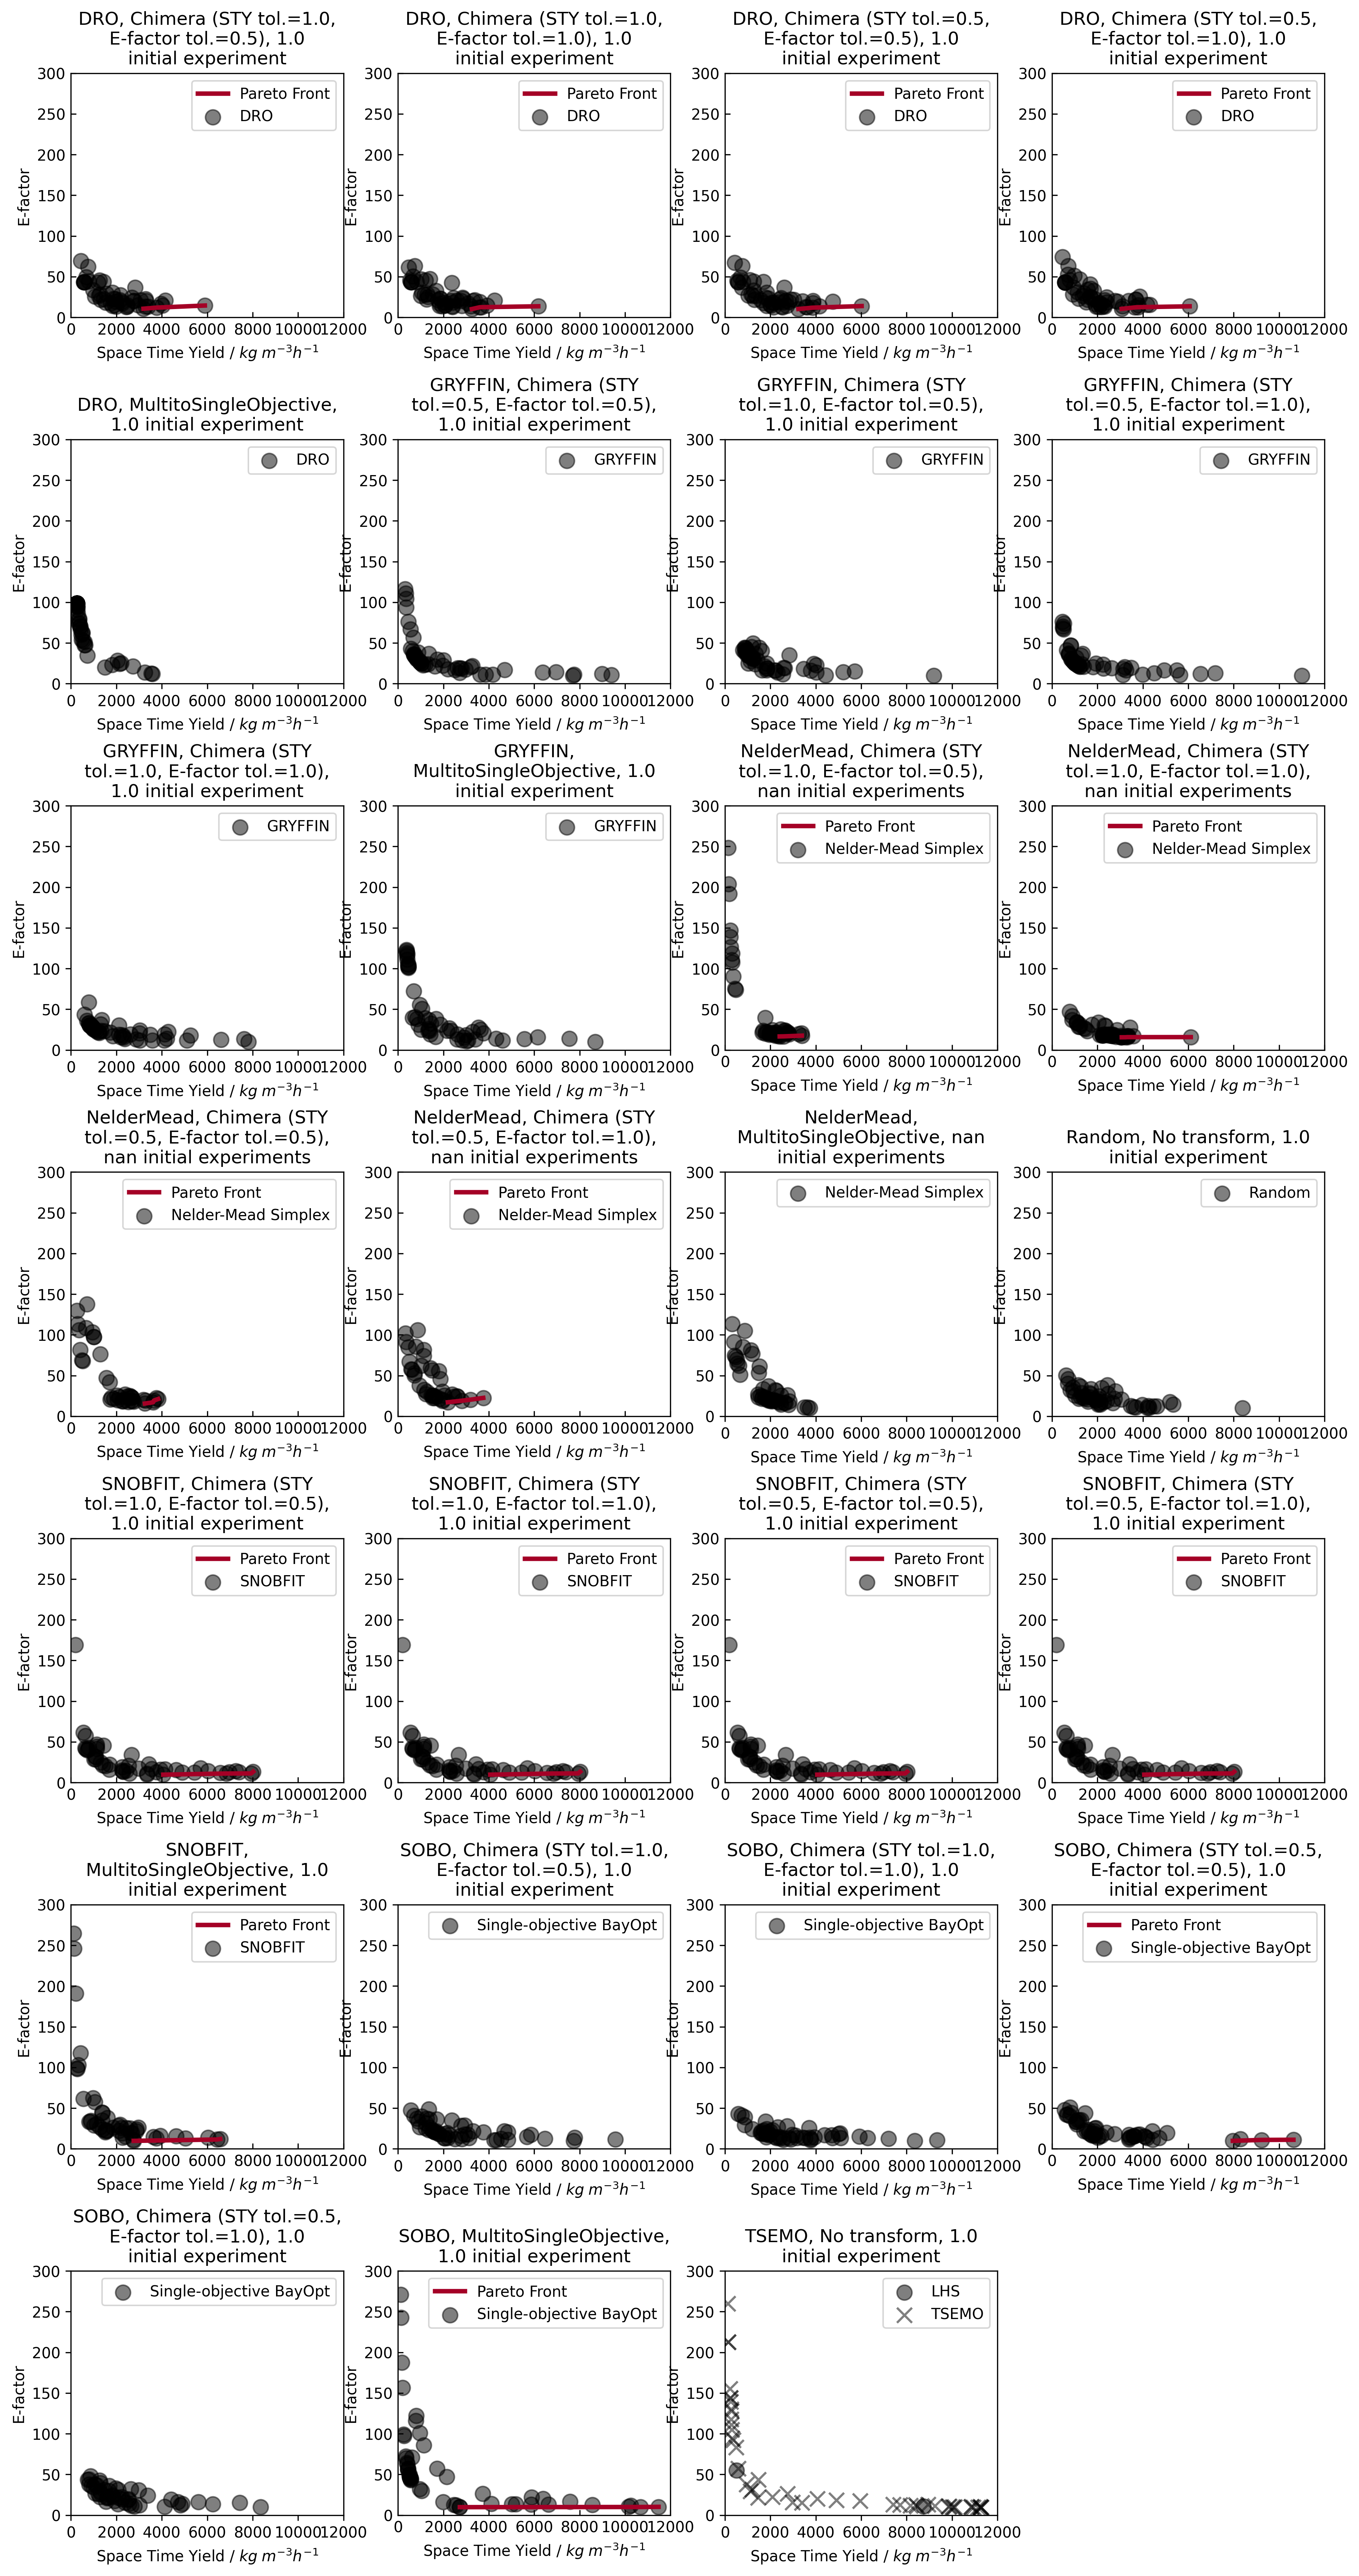
\includegraphics[height=0.8\textheight]{gfx/Appendix/snar_pareto_fronts.png}
    \caption{Pareto fronts for the best run (by terminal hypervolume) of each unique combination of strategy, transform, and number of initial experiments for the SnAr benchmark.}
    \label{fig:snar_pareto_fronts}
\end{figure}


\begin{table}[]
    \centering
    \begin{tabular}{lllllll}
        \textbf{Strategy} & \textbf{Transform} & \textbf{STY tol.} & \textbf{E-factor tol. }& \textbf{Hypervolume} & \textbf{Time (s) }  & \textbf{Repeats}                \\
        \hline
        DRO & Chimera & 0.5 & 0.5 &        10.0$\pm$29.0 &        0.0$\pm$0.0 &       20 \\
              &           &     & 1.0 &          2.0$\pm$7.0 &        0.0$\pm$0.0 &       20 \\
              &           & 1.0 & 0.5 &          0.0$\pm$2.0 &        0.0$\pm$0.0 &       20 \\
              &           &     & 1.0 &         7.0$\pm$29.0 &        0.0$\pm$0.0 &       20 \\
              & Custom & - & - &          0.0$\pm$0.0 &        0.0$\pm$0.0 &       20 \\
        GRYFFIN & Chimera & 0.5 & 0.5 &     669.0$\pm$1132.0 &      79.0$\pm$11.0 &       20 \\
              &           &     & 1.0 &    1449.0$\pm$2243.0 &      78.0$\pm$11.0 &       20 \\
              &           & 1.0 & 0.5 &    1715.0$\pm$1766.0 &     106.0$\pm$19.0 &       20 \\
              &           &     & 1.0 &    1959.0$\pm$1545.0 &      87.0$\pm$12.0 &       20 \\
              & Custom & - & - &     528.0$\pm$1048.0 &      89.0$\pm$10.0 &       20 \\
        NelderMead & Chimera & 0.5 & 0.5 &          0.0$\pm$0.0 &        0.0$\pm$0.0 &       20 \\
              &           &     & 1.0 &          0.0$\pm$0.0 &        0.0$\pm$0.0 &       20 \\
              &           & 1.0 & 0.5 &          0.0$\pm$0.0 &        0.0$\pm$0.0 &       20 \\
              &           &     & 1.0 &          0.0$\pm$0.0 &        0.0$\pm$0.0 &       20 \\
              & Custom & - & - &       43.0$\pm$108.0 &        0.0$\pm$0.0 &       20 \\
        Random & Transform & - & - &    1032.0$\pm$1315.0 &        0.0$\pm$0.0 &       20 \\
        SNOBFIT & Chimera & 0.5 & 0.5 &       1095.0$\pm$0.0 &        0.0$\pm$0.0 &       20 \\
              &           &     & 1.0 &       1095.0$\pm$0.0 &        0.0$\pm$0.0 &       20 \\
              &           & 1.0 & 0.5 &       1095.0$\pm$0.0 &        0.0$\pm$0.0 &       20 \\
              &           &     & 1.0 &       1095.0$\pm$0.0 &        0.0$\pm$0.0 &       20 \\
              & Custom & - & - &          0.0$\pm$0.0 &        0.0$\pm$0.0 &       20 \\
        SOBO & Chimera & 0.5 & 0.5 &     634.0$\pm$1049.0 &        0.0$\pm$0.0 &       20 \\
              &           &     & 1.0 &      593.0$\pm$876.0 &        0.0$\pm$0.0 &       20 \\
              &           & 1.0 & 0.5 &    1414.0$\pm$1599.0 &        0.0$\pm$0.0 &       20 \\
              &           &     & 1.0 &     786.0$\pm$1325.0 &        0.0$\pm$0.0 &       20 \\
              & Custom & - & - &    2013.0$\pm$2155.0 &        0.0$\pm$0.0 &       20 \\
        TSEMO & Transform & - & - &    5803.0$\pm$2659.0 &       42.0$\pm$1.0 &       20 \\
    \end{tabular}
    \caption{Results of tests of strategies and transforms available in Summit on the SnAr benchmark. Each strategy and transform combination was run with twenty repeats and results are shown with the standard deviation.}
    \label{tab:snar_benchmark_results}
\end{table}


\subsection{C-N Benchmark details as implemented for the Summit paper}


 The cost is determined using data from chemical suppliers, as shown in \ref{tab:cn_benchmark_prices_1} and \ref{tab:cn_benchmark_prices_2}. For the bases, we use data supplied by Baumgartner et al.\cite{Baumgartner2019}, and all other data is determined by us.
 
\begin{sidewaystable}[]
\caption{Chemicals used in C-N Benchmark.}
\begin{tabular}{ccccc}
\textbf{Abbreviation}             & \textbf{MW (g/mol)} & \textbf{Density (g/mL)} & \textbf{CAS Number} & \textbf{Supplier} \\
\hline
t-BuXPhos     & 686.69 & -     & 1142811-12-8 & Sigma-Alddrich (Merck) \\
t-BuBrettPhos & 854.43 & -     & 1536473-72-9 & Sigma-Alddrich (Merck) \\
AlPhos        & 815.06 & -     & 2097600-15-0 & Sigma-Alddrich (Merck) \\
p-Tolyl TMS   & 240.2               & -                       & 29540-83-8          & TCI Chemicals     \\
Anniline      & 93.13  & 1.022 & 62-53-3      & Sigma-Alddrich (Merck) \\
TEA           & 101.19 & 0.726 & 121-44-8     & Millipore-Sigma        \\
TMG           & 115.18 & 0.918 & 80-70-6      & BetaPharma             \\
BTMG          & 171.28 & 0.85  & 29166-72-1   & BetaPharma             \\
DBU           & 152.24 & 1.018 & 6674-22-2    & ChemShuttle            \\
MTBD          & 153.22 & 1.067 & 84030-20-6   & Enamine BB             \\
BTTP          & 312.43 & 1.022 & 161118-67-8  & Millipore-Sigma        \\
P2Et          & 339.4  & 1.02  & 165535-45-5  & Millipore-Sigma       
\end{tabular}
\label{tab:cn_benchmark_prices_1}
\end{sidewaystable}

\begin{sidewaystable}[]
\caption{Prices of compounds used in C-N benchmark.}
\begin{tabular}{ccccc}
\textbf{Abbreviation} & \textbf{Mass Available (g)} & \textbf{Volume Availability (mL)} & \textbf{Price} & \textbf{Price /mmol} \\
\hline
t-BuXPhos     & 1        & -        & \$137.00   & \$94.08  \\
t-BuBrettPhos & 5        & -        & \$1,070.00 & \$182.85 \\
AlPhos        & 1        & -        & \$729.00   & \$594.18 \\
p-Tolyl TMS   & 5        & -        & \$123.00   & \$5.91   \\
Anniline      & -        & 1000     & \$109.00   & \$0.01   \\
TEA           & 20000    & 143492.4 & \$1,830.00 & \$0.01   \\
TMG           & 21786.49 & 173641.3 & \$184.00   & \$0.00   \\
BTMG          & 117.65   & 583.8    & \$706.00   & \$1.21   \\
DBU           & 4911.59  & 32842.9  & \$893.00   & \$0.03   \\
MTBD          & 9.37     & 65.3     & \$511.00   & \$7.83   \\
BTTP          & 25       & 81.8     & \$572.00   & \$6.99   \\
P2Et          & 5        & 15       & \$601.00   & \$40.00 
\end{tabular}

\label{tab:cn_benchmark_prices_2}
\end{sidewaystable}

\ref{fig:cn_pareto_fronts} displays the pareto fronts of the best performing run from each combination of strategy and transform, while \ref{tab:cn_benchmark} enumerates the results of the tests of the C-N benchmark. Note that for the Custom multi-objective transform, the following expression was minimized: $-yield+cost$.

\begin{figure}[p]
    \centering
    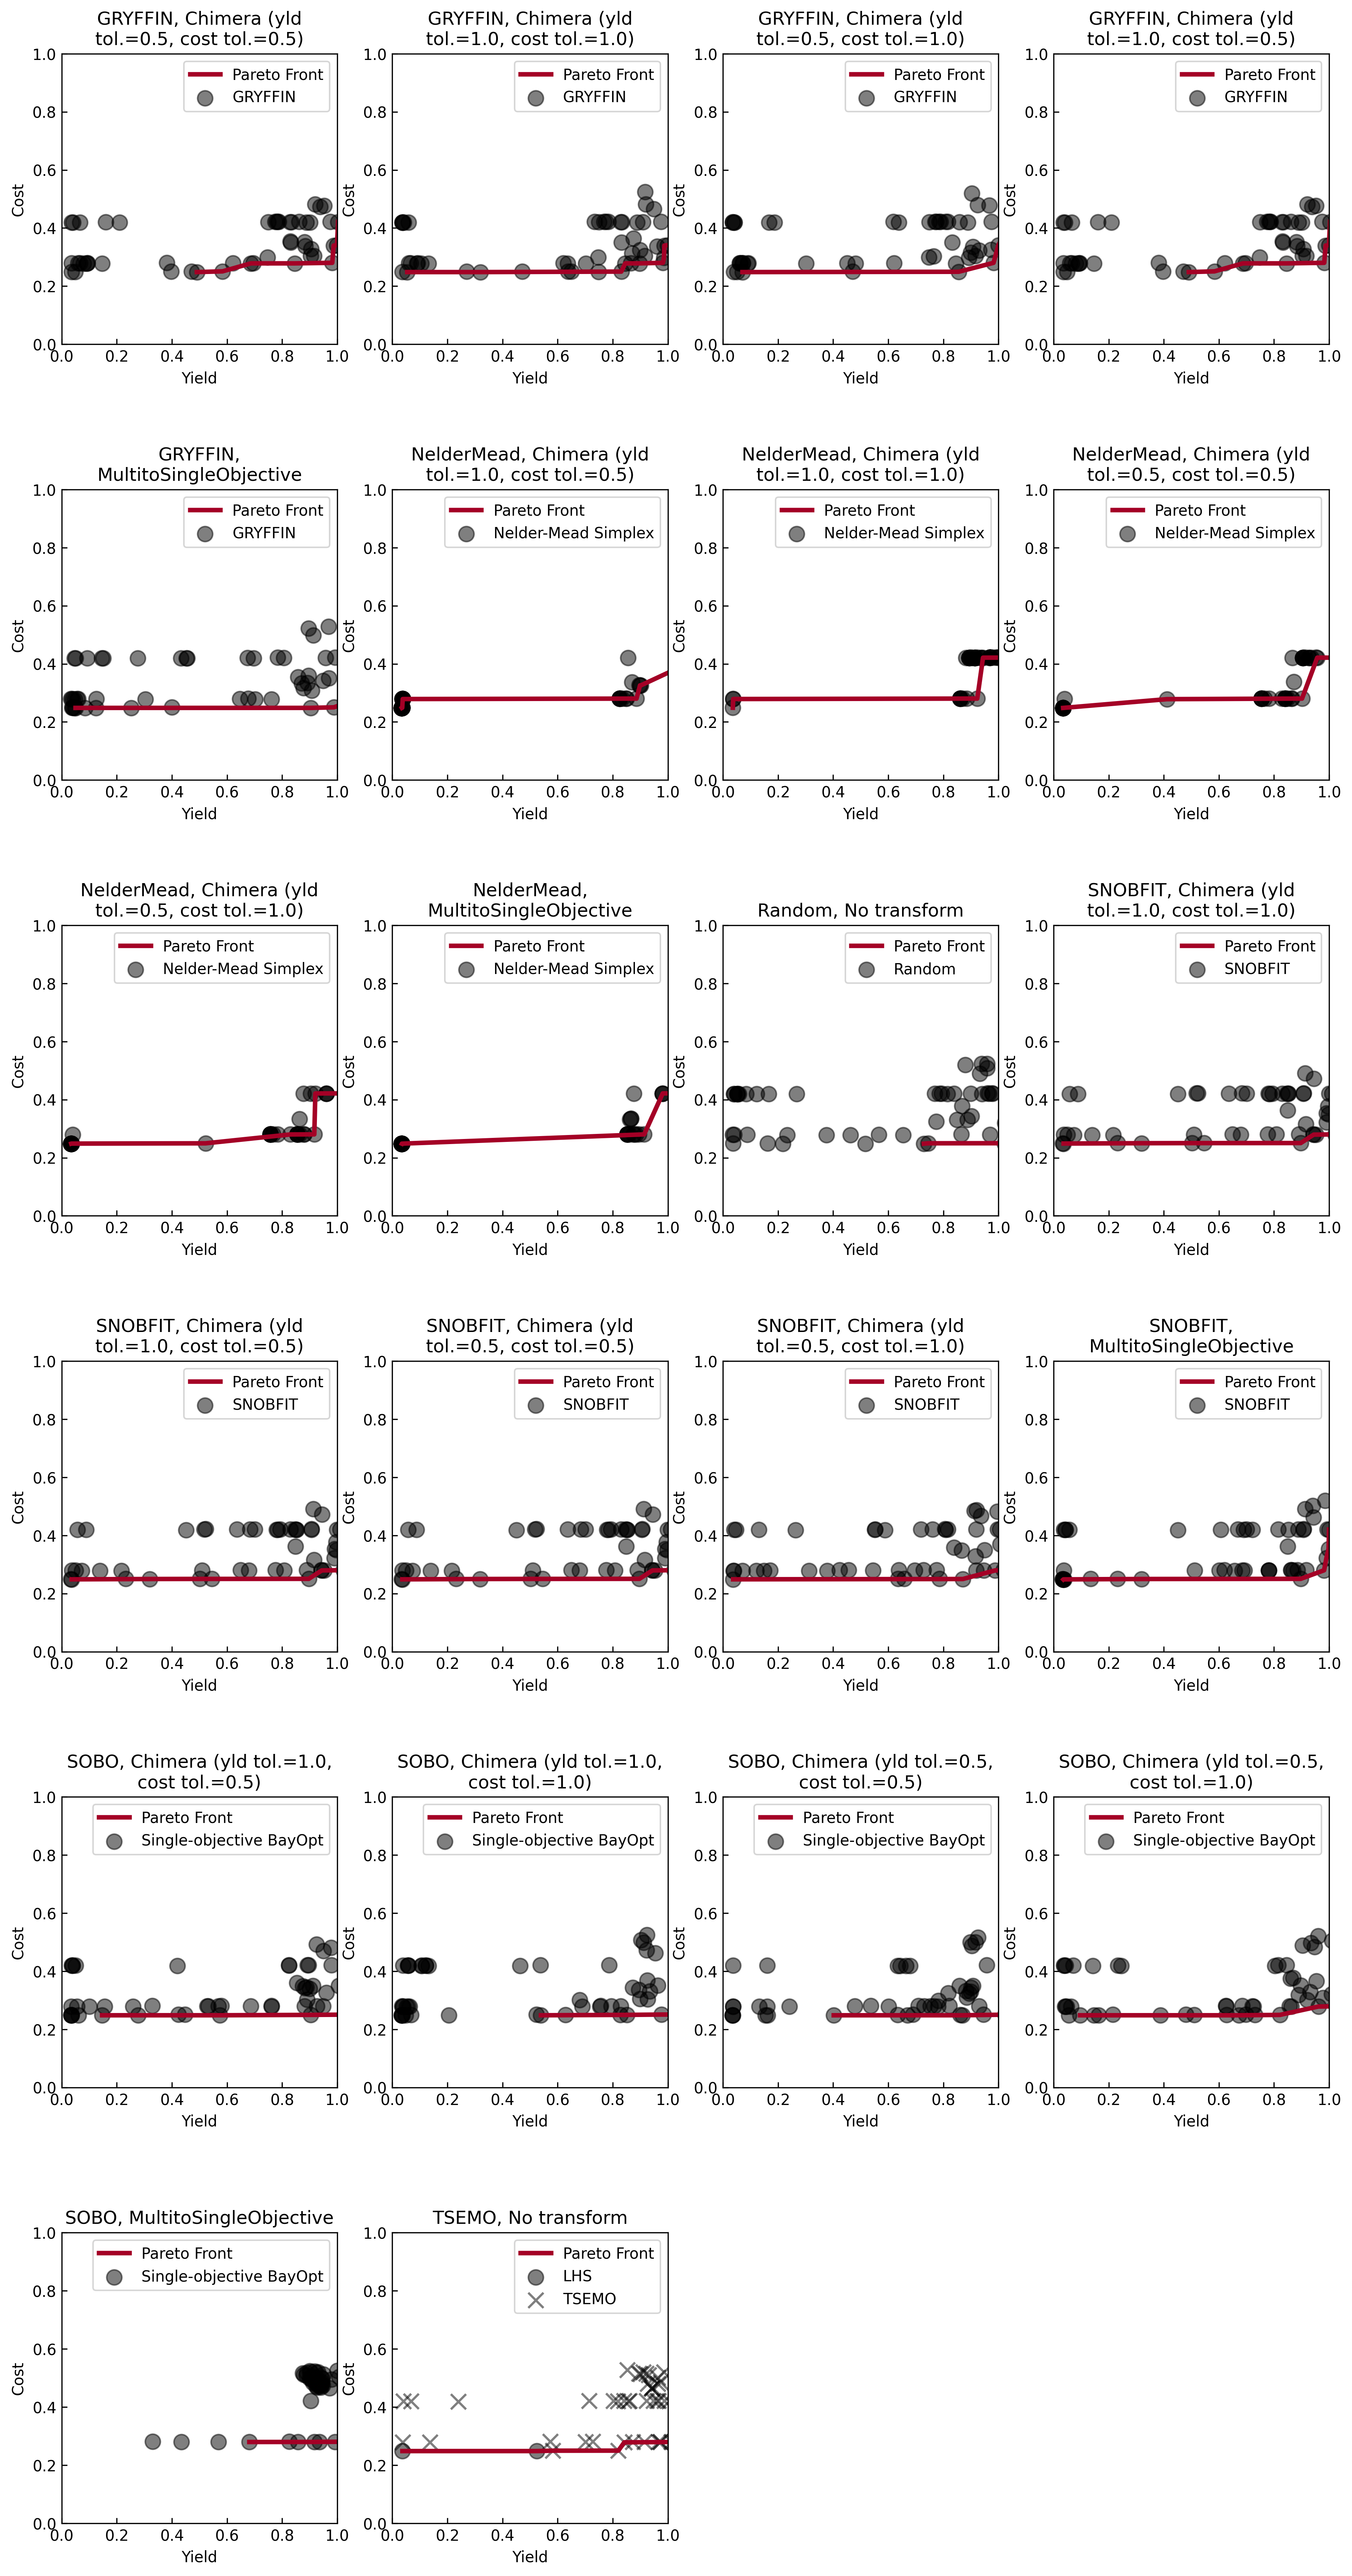
\includegraphics[height=0.8\textheight]{gfx/Appendix/cn_pareto_fronts.png}
    \caption{Pareto fronts for the best run (by terminal hypervolume) of each unique combination of strategy, transform, and number of initial experiments for the CN benchmark.}
    \label{fig:cn_pareto_fronts}
\end{figure}

\begin{table}[]
    \centering
    \begin{tabular}{lllllll}
        \textbf{Strategy} & \textbf{Transform} & \textbf{Yield tol.} & \textbf{Cost tol. }& \textbf{Hypervolume} & \textbf{Time (s) }  & \textbf{Repeats}                \\
        \hline
        GRYFFIN & Chimera & 0.5 & 0.5 &         0.74$\pm$0.0 &     15.13$\pm$0.52 &       20 \\
              &           &     & 1.0 &        0.74$\pm$0.01 &     16.57$\pm$4.38 &       20 \\
              &           & 1.0 & 0.5 &         0.74$\pm$0.0 &     13.64$\pm$0.61 &       20 \\
              &           &     & 1.0 &         0.74$\pm$0.0 &     14.35$\pm$1.25 &       20 \\
              & Custom & - & - &        0.77$\pm$0.02 &     34.21$\pm$1.95 &       20 \\
        NelderMead & Chimera & 0.5 & 0.5 &        0.73$\pm$0.05 &       0.03$\pm$0.0 &       20 \\
              &           &     & 1.0 &        0.72$\pm$0.05 &      0.04$\pm$0.01 &       20 \\
              &           & 1.0 & 0.5 &        0.72$\pm$0.05 &      0.04$\pm$0.01 &       20 \\
              &           &     & 1.0 &        0.72$\pm$0.05 &      0.03$\pm$0.01 &       20 \\
              & Custom & - & - &        0.73$\pm$0.05 &      0.04$\pm$0.01 &       20 \\
        Random & Transform & - & - &        0.76$\pm$0.03 &       0.02$\pm$0.0 &       20 \\
        SNOBFIT & Chimera & 0.5 & 0.5 &         0.79$\pm$0.0 &       0.05$\pm$0.0 &       20 \\
              &           &     & 1.0 &        0.79$\pm$0.01 &      0.06$\pm$0.03 &       20 \\
              &           & 1.0 & 0.5 &         0.79$\pm$0.0 &       0.05$\pm$0.0 &       20 \\
              &           &     & 1.0 &         0.79$\pm$0.0 &       0.04$\pm$0.0 &       20 \\
              & Custom & - & - &         0.75$\pm$0.0 &       0.06$\pm$0.0 &       20 \\
        SOBO & Chimera & 0.5 & 0.5 &        0.76$\pm$0.03 &      0.14$\pm$0.01 &       20 \\
              &           &     & 1.0 &        0.76$\pm$0.02 &      0.15$\pm$0.01 &       20 \\
              &           & 1.0 & 0.5 &        0.76$\pm$0.03 &      0.15$\pm$0.01 &       20 \\
              &           &     & 1.0 &        0.76$\pm$0.03 &      0.14$\pm$0.01 &       20 \\
              & Custom & - & - &        0.71$\pm$0.03 &      0.24$\pm$0.02 &       20 \\
        TSEMO & Transform & - & - &        0.79$\pm$0.02 &   182.96$\pm$16.11 &       20 \\
    \end{tabular}
    \caption{Results of tests of strategies and transforms available in Summit on the CN benchmark. Each strategy and transform combination was run with twenty repeats and results are shown with the standard deviation. tol. stands for the tolerance used in Chimera where applicable, time is is the average time per iteration for a new suggestion from the strategy.}
    \label{tab:cn_benchmark}
\end{table}

\section{Multi-task benchmarks additional data}

\begin{figure}
\caption{Parity plot of benchmark training for prediction of reaction yield for C-N B1.}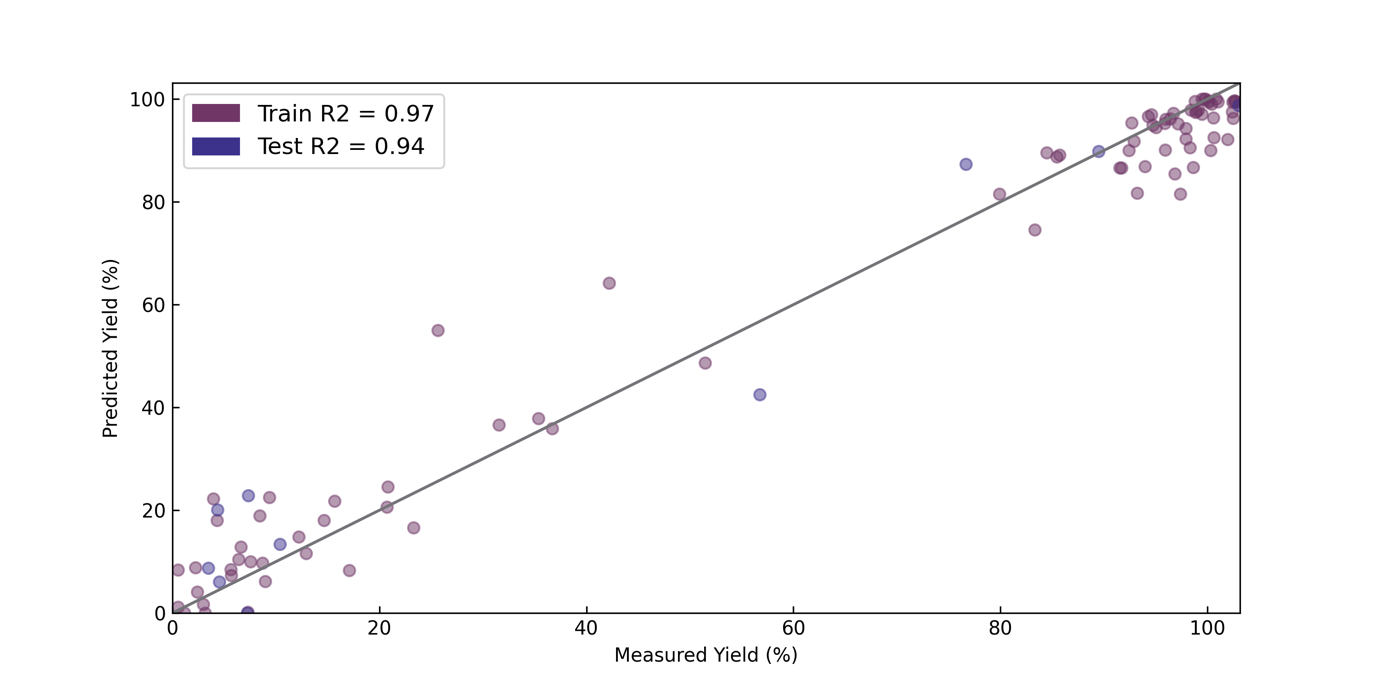
\includegraphics[width=1\textwidth]{gfx/Appendix/baumgartner_cn_case_1_parity_plot.png}
\label{fig:1}
\end{figure}

\begin{figure}
\caption{ Parity plot of benchmark training for prediction of reaction yield for C-N B2.}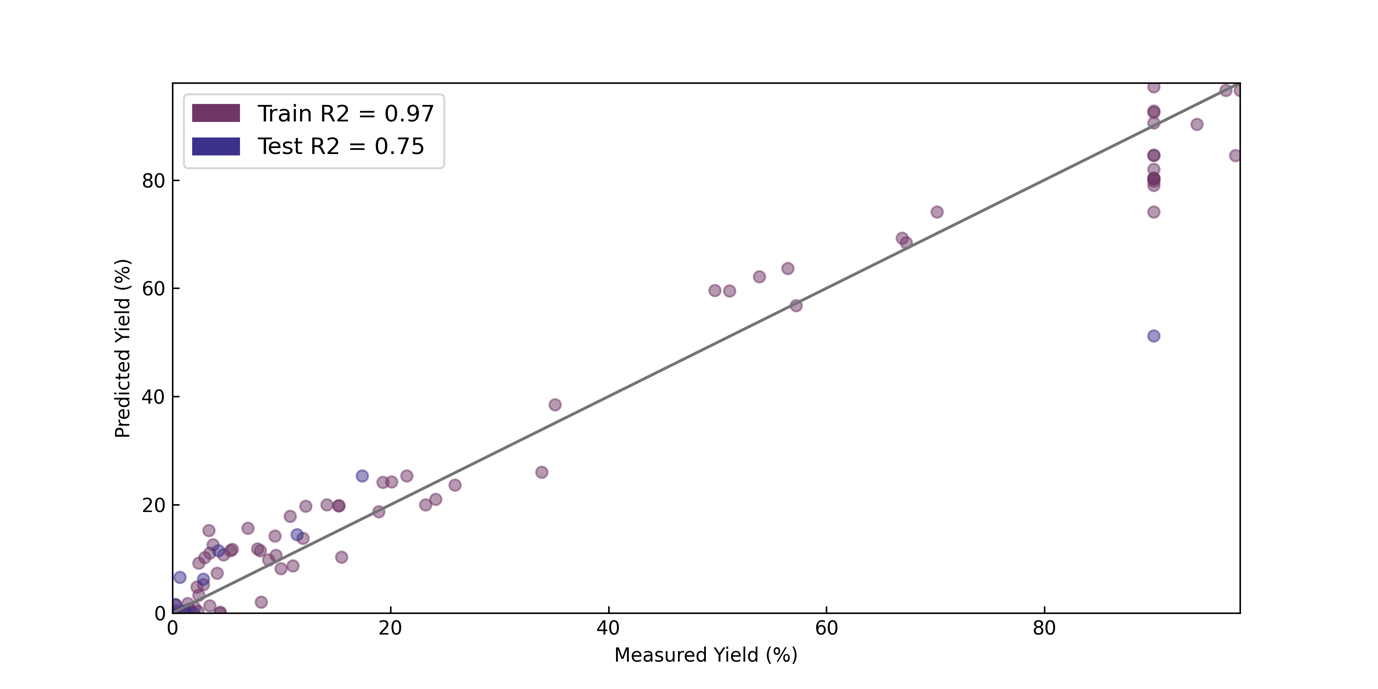
\includegraphics[width=1\textwidth]{gfx/Appendix/baumgartner_cn_case_2_parity_plot.png}
\label{fig:2}
\end{figure}

\begin{figure}
\caption{Parity plot of benchmark training for prediction of reaction yield for C-N B3.}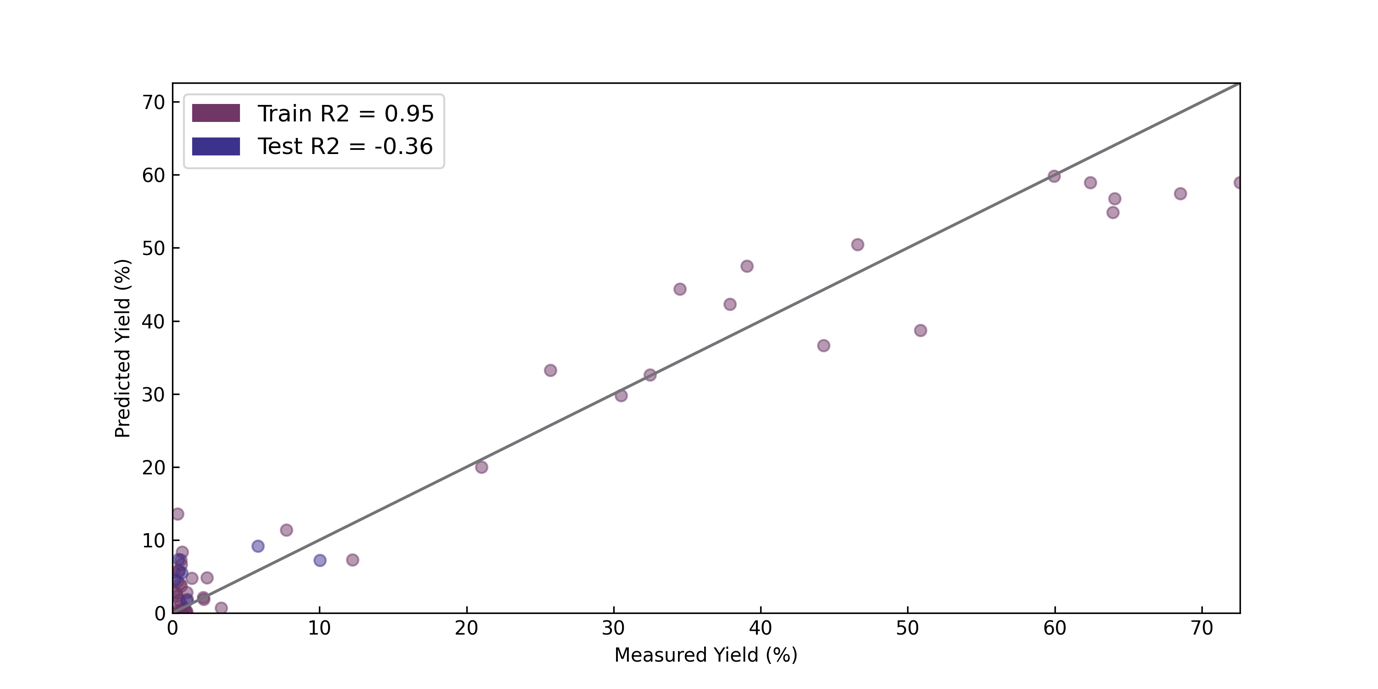
\includegraphics[width=1\textwidth]{gfx/Appendix/baumgartner_cn_case_3_parity_plot.png}
\label{fig:3}
\end{figure}

\begin{figure}
\caption{Parity plot of benchmark training for prediction of reaction yield for C-N B4.}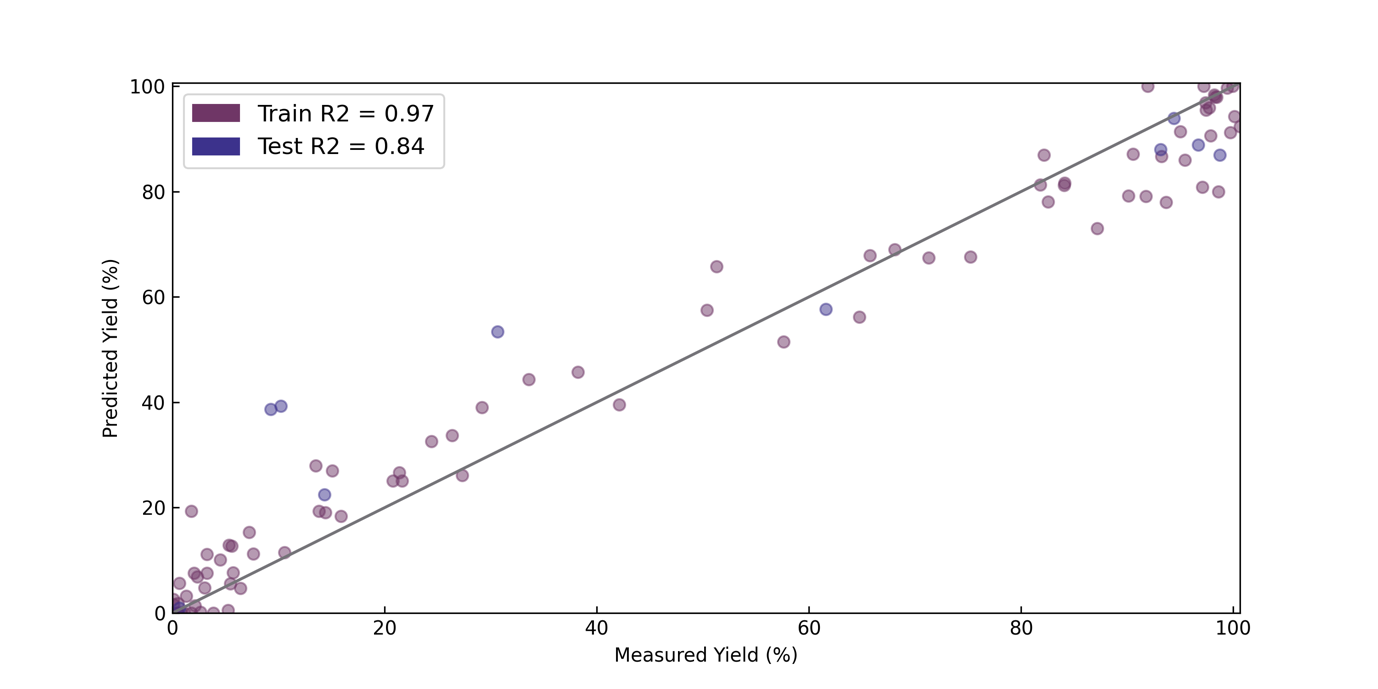
\includegraphics[width=1\textwidth]{gfx/Appendix/baumgartner_cn_case_4_parity_plot.png}
\label{fig:4}
\end{figure}

\begin{figure}
\caption{ Parity plot of benchmark training for prediction of reaction yield for Suzuki B1.}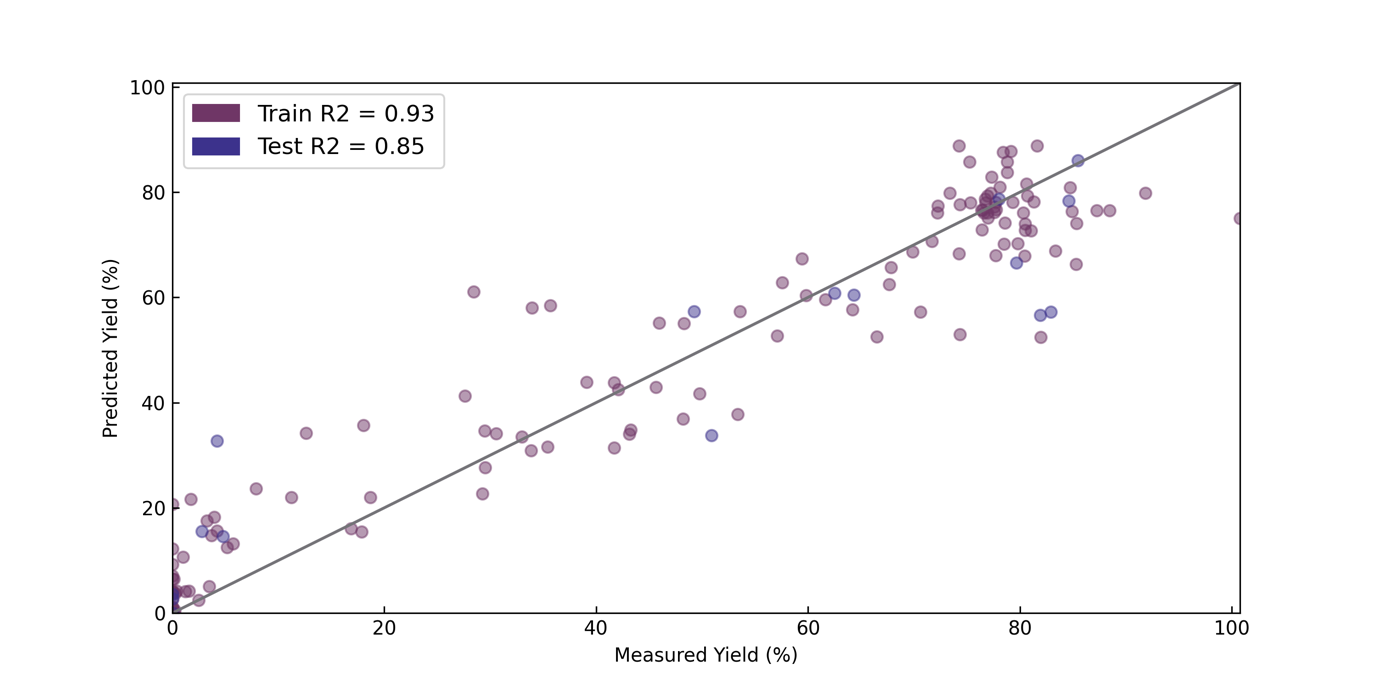
\includegraphics[width=1\textwidth]{gfx/Appendix/baumgartner_suzuki_parity_plot.png}
\label{fig:5}
\end{figure}

\begin{figure}
\caption{Parity plot of benchmark training for prediction of reaction yield for Suzuki R1.}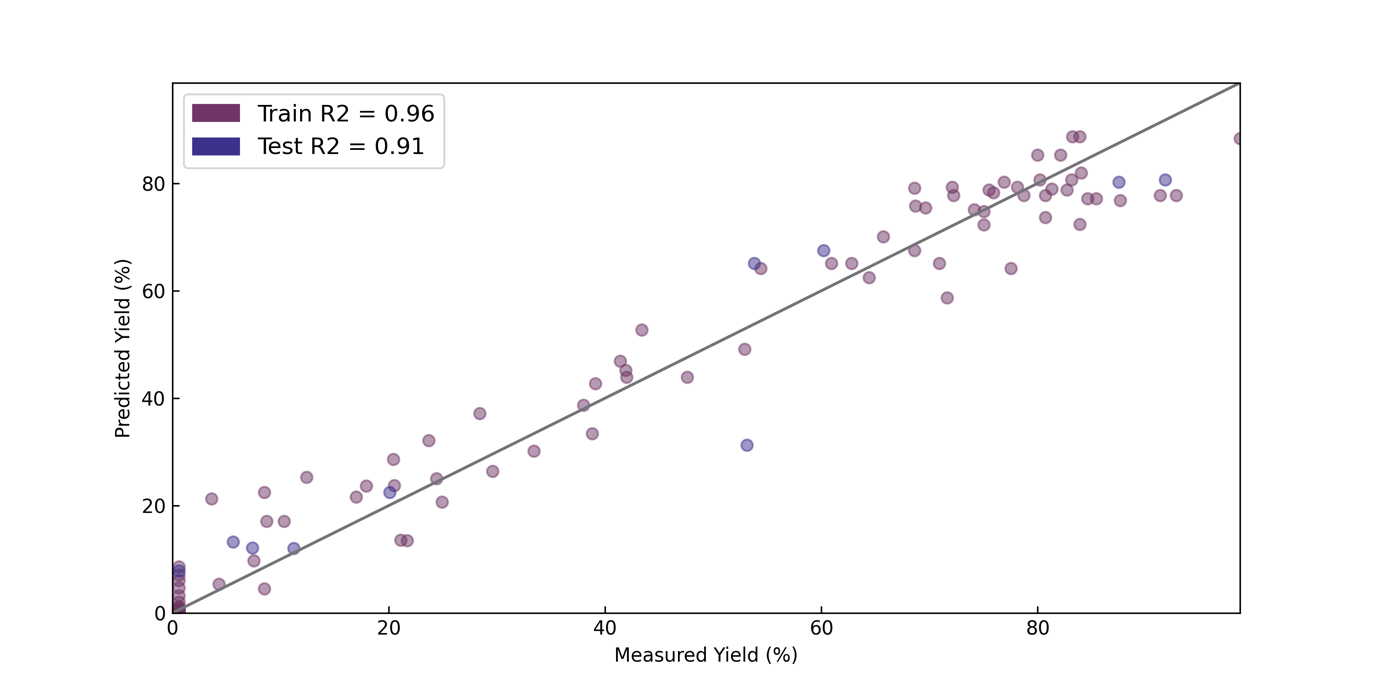
\includegraphics[width=1\textwidth]{gfx/Appendix/reizman_suzuki_case_1_parity_plot.png}
\label{fig:6}
\end{figure}

\begin{figure}
\caption{ Parity plot of benchmark training for prediction of reaction yield for Suzuki R2.}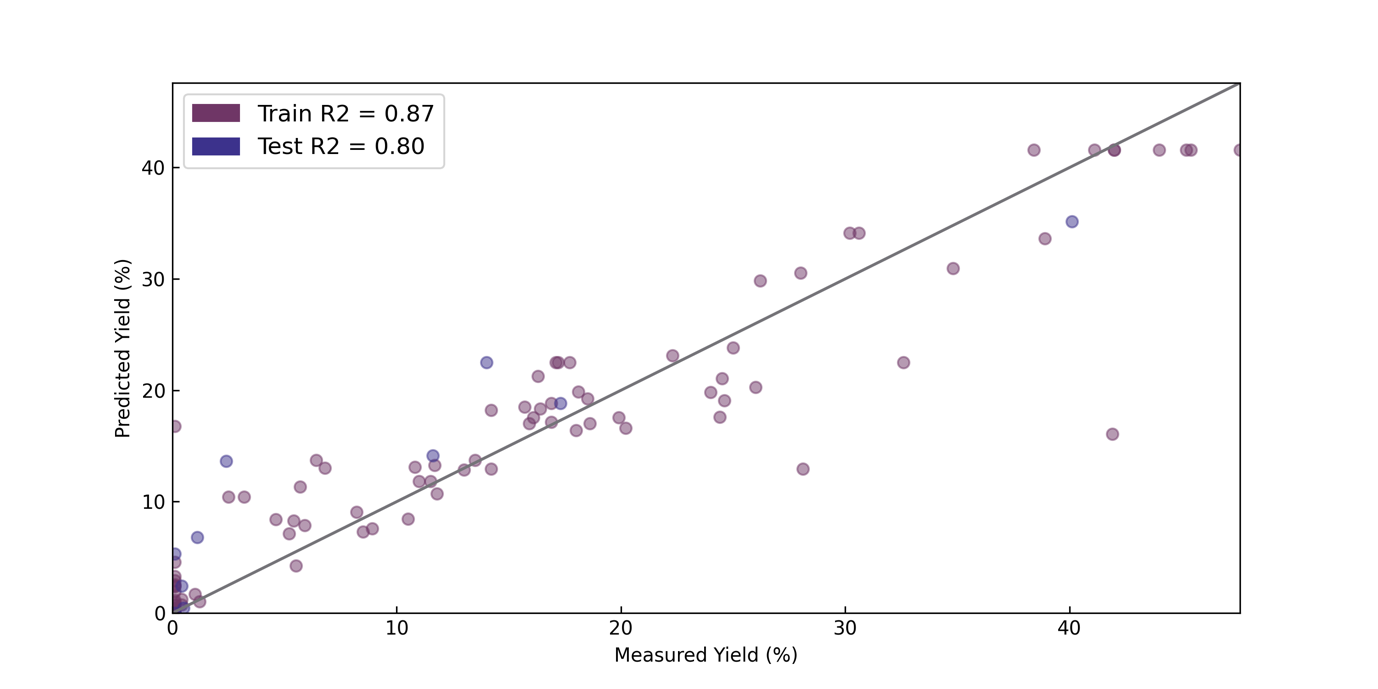
\includegraphics[width=1\textwidth]{gfx/Appendix/reizman_suzuki_case_2_parity_plot.png}
\label{fig:7}
\end{figure}

\begin{figure}
\caption{Parity plot of benchmark training for prediction of reaction yield for Suzuki R3.}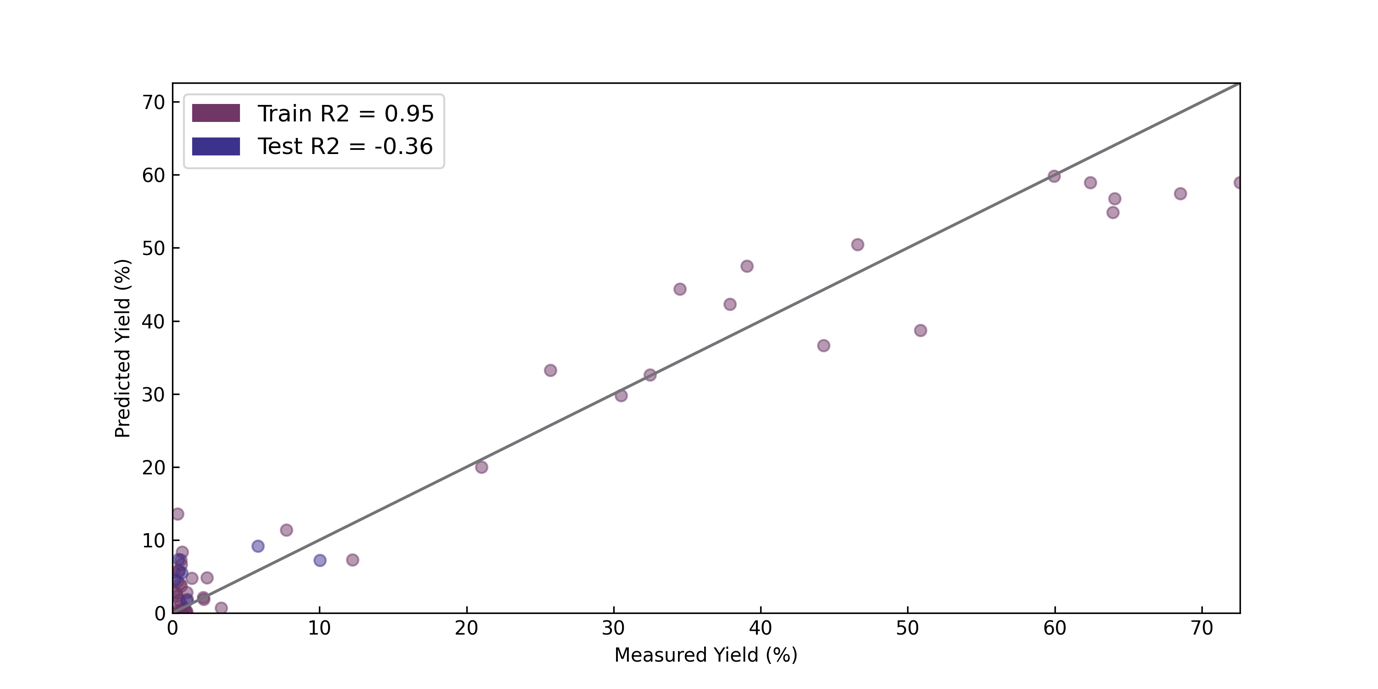
\includegraphics[width=1\textwidth]{gfx/Appendix/baumgartner_cn_case_3_parity_plot.png}
\label{fig:8}
\end{figure}

\begin{figure}
\caption{Parity plot of benchmark training for prediction of reaction yield for Suzuki R4.}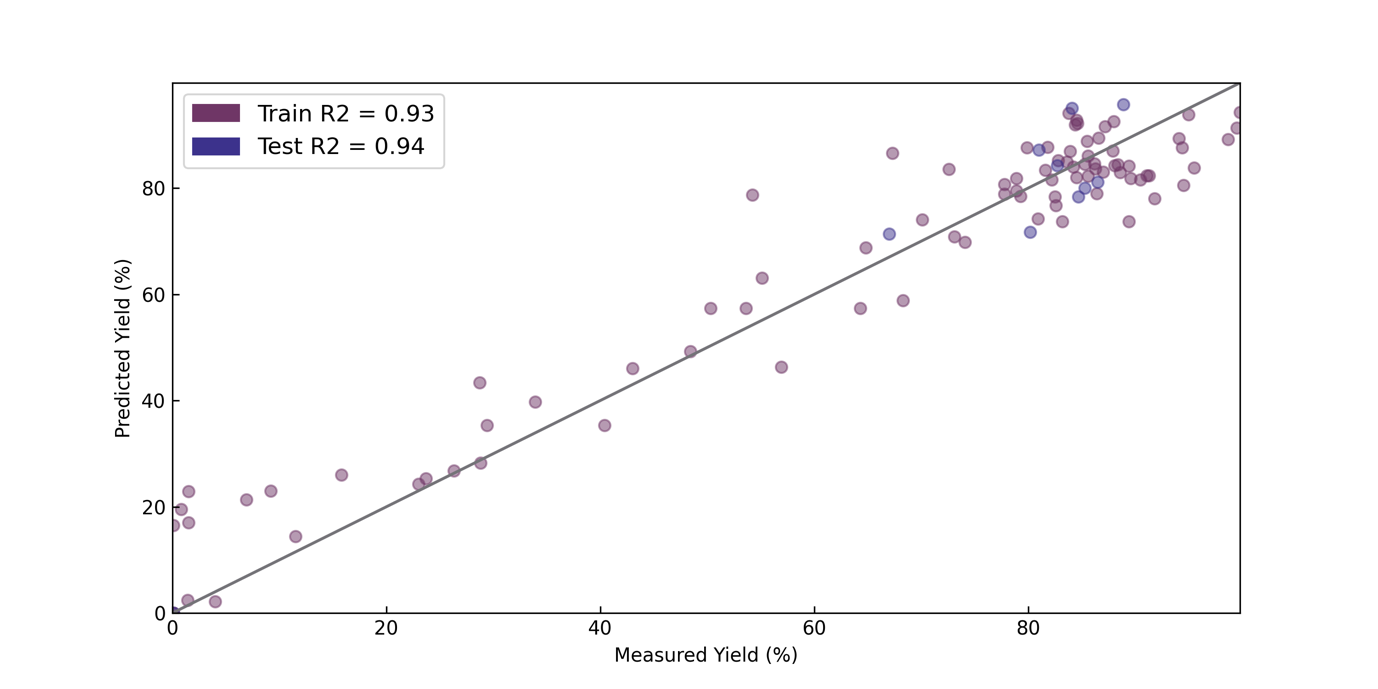
\includegraphics[width=1\textwidth]{gfx/Appendix/reizman_suzuki_case_4_parity_plot.png}
\label{fig:9}
\end{figure}


\subsection{Suzuki Benchmarks}

\begin{figure}
\caption{ Comparison of the performance of single-task Bayesian optimization (STBO) and multi-task Bayesian optimization (MTBO) on Suzuki reactions R1-R4 with auxiliary data from Suzuki B1.}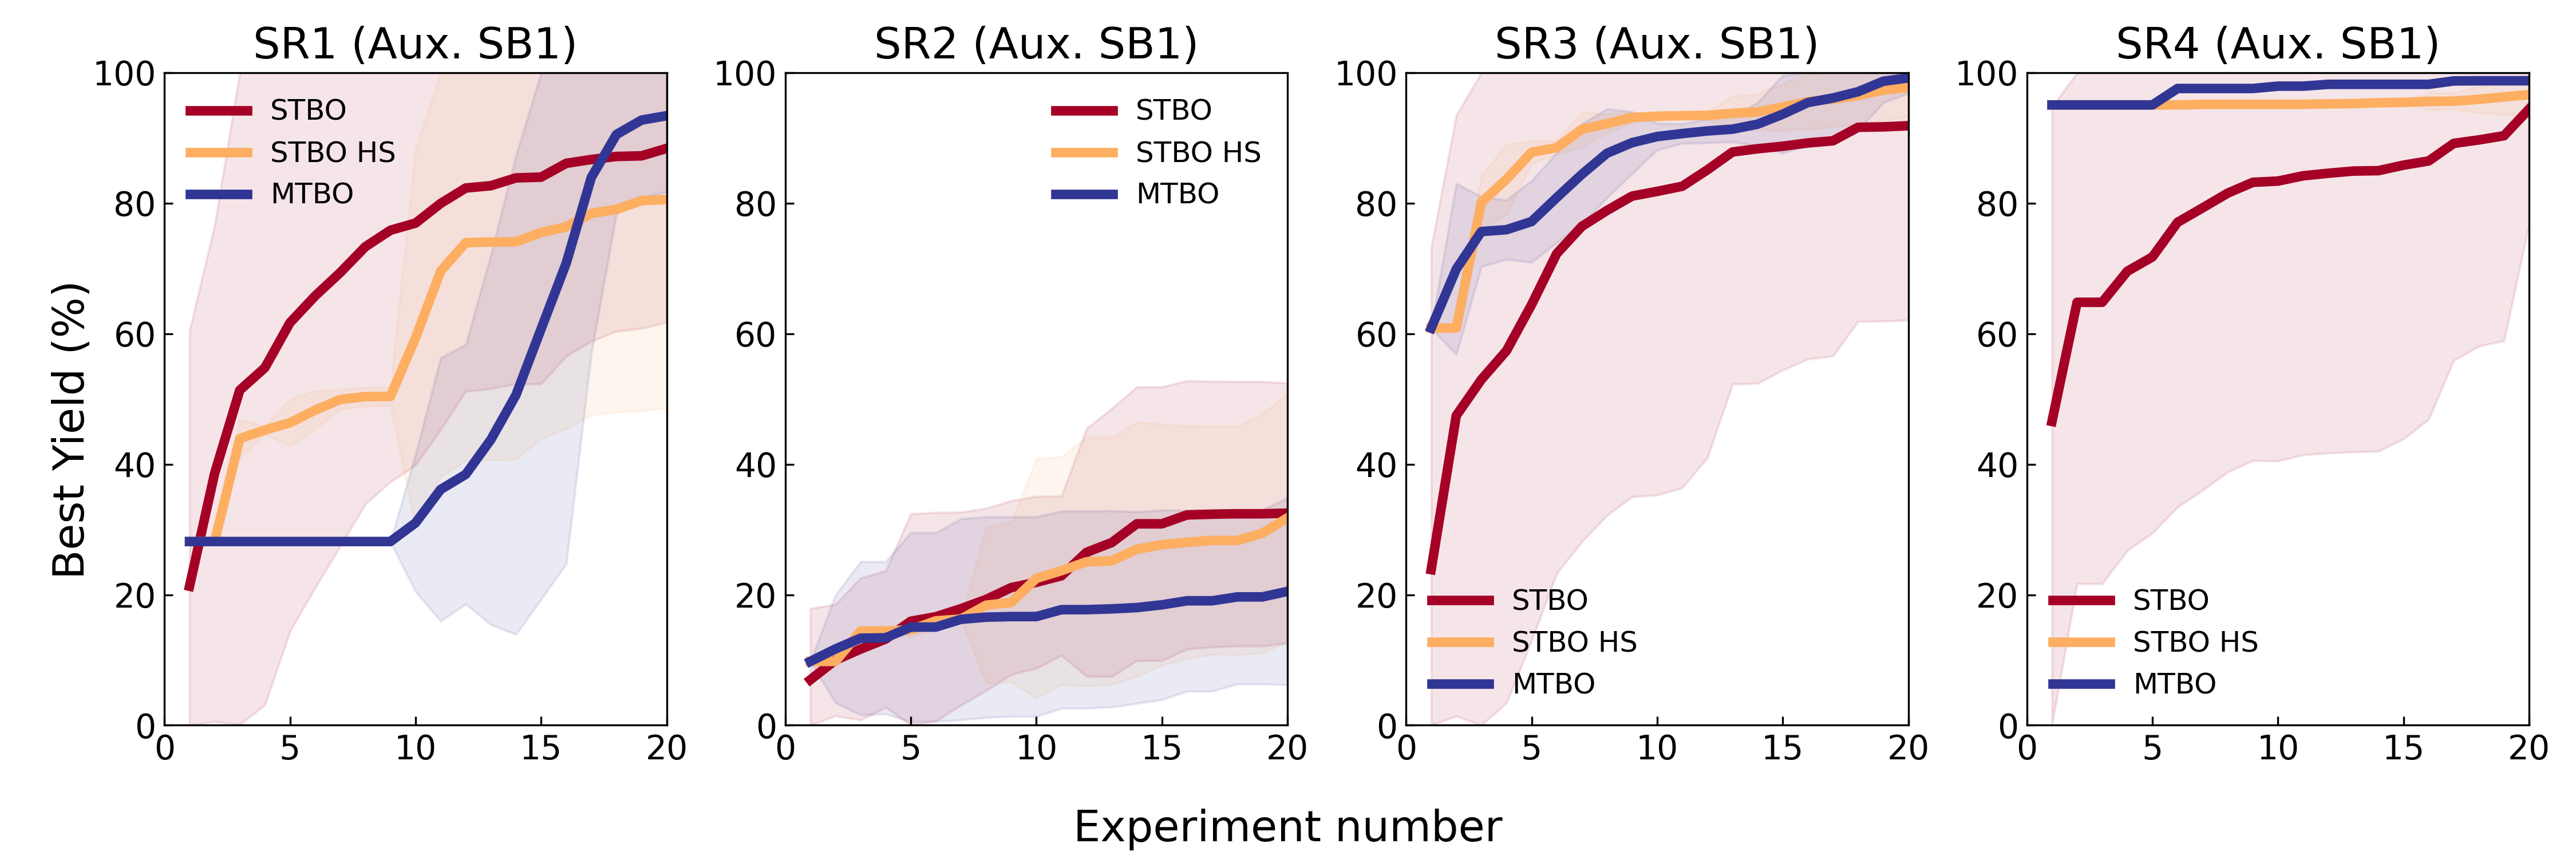
\includegraphics[width=1\textwidth]{gfx/Appendix/reizman_suzuki_baumgartner_suzuki_one_cotraining_optimization.png}
\label{fig:10}
\end{figure}

\begin{figure}
\caption{Comparison of the performance of single-task Bayesian optimization (STBO) and multi-task Bayesian optimization (MTBO) on Suzuki R1-R4 with Suzuki R1-R4 as auxiliary tasks. The text above the plot represents the data used as an auxiliary task.}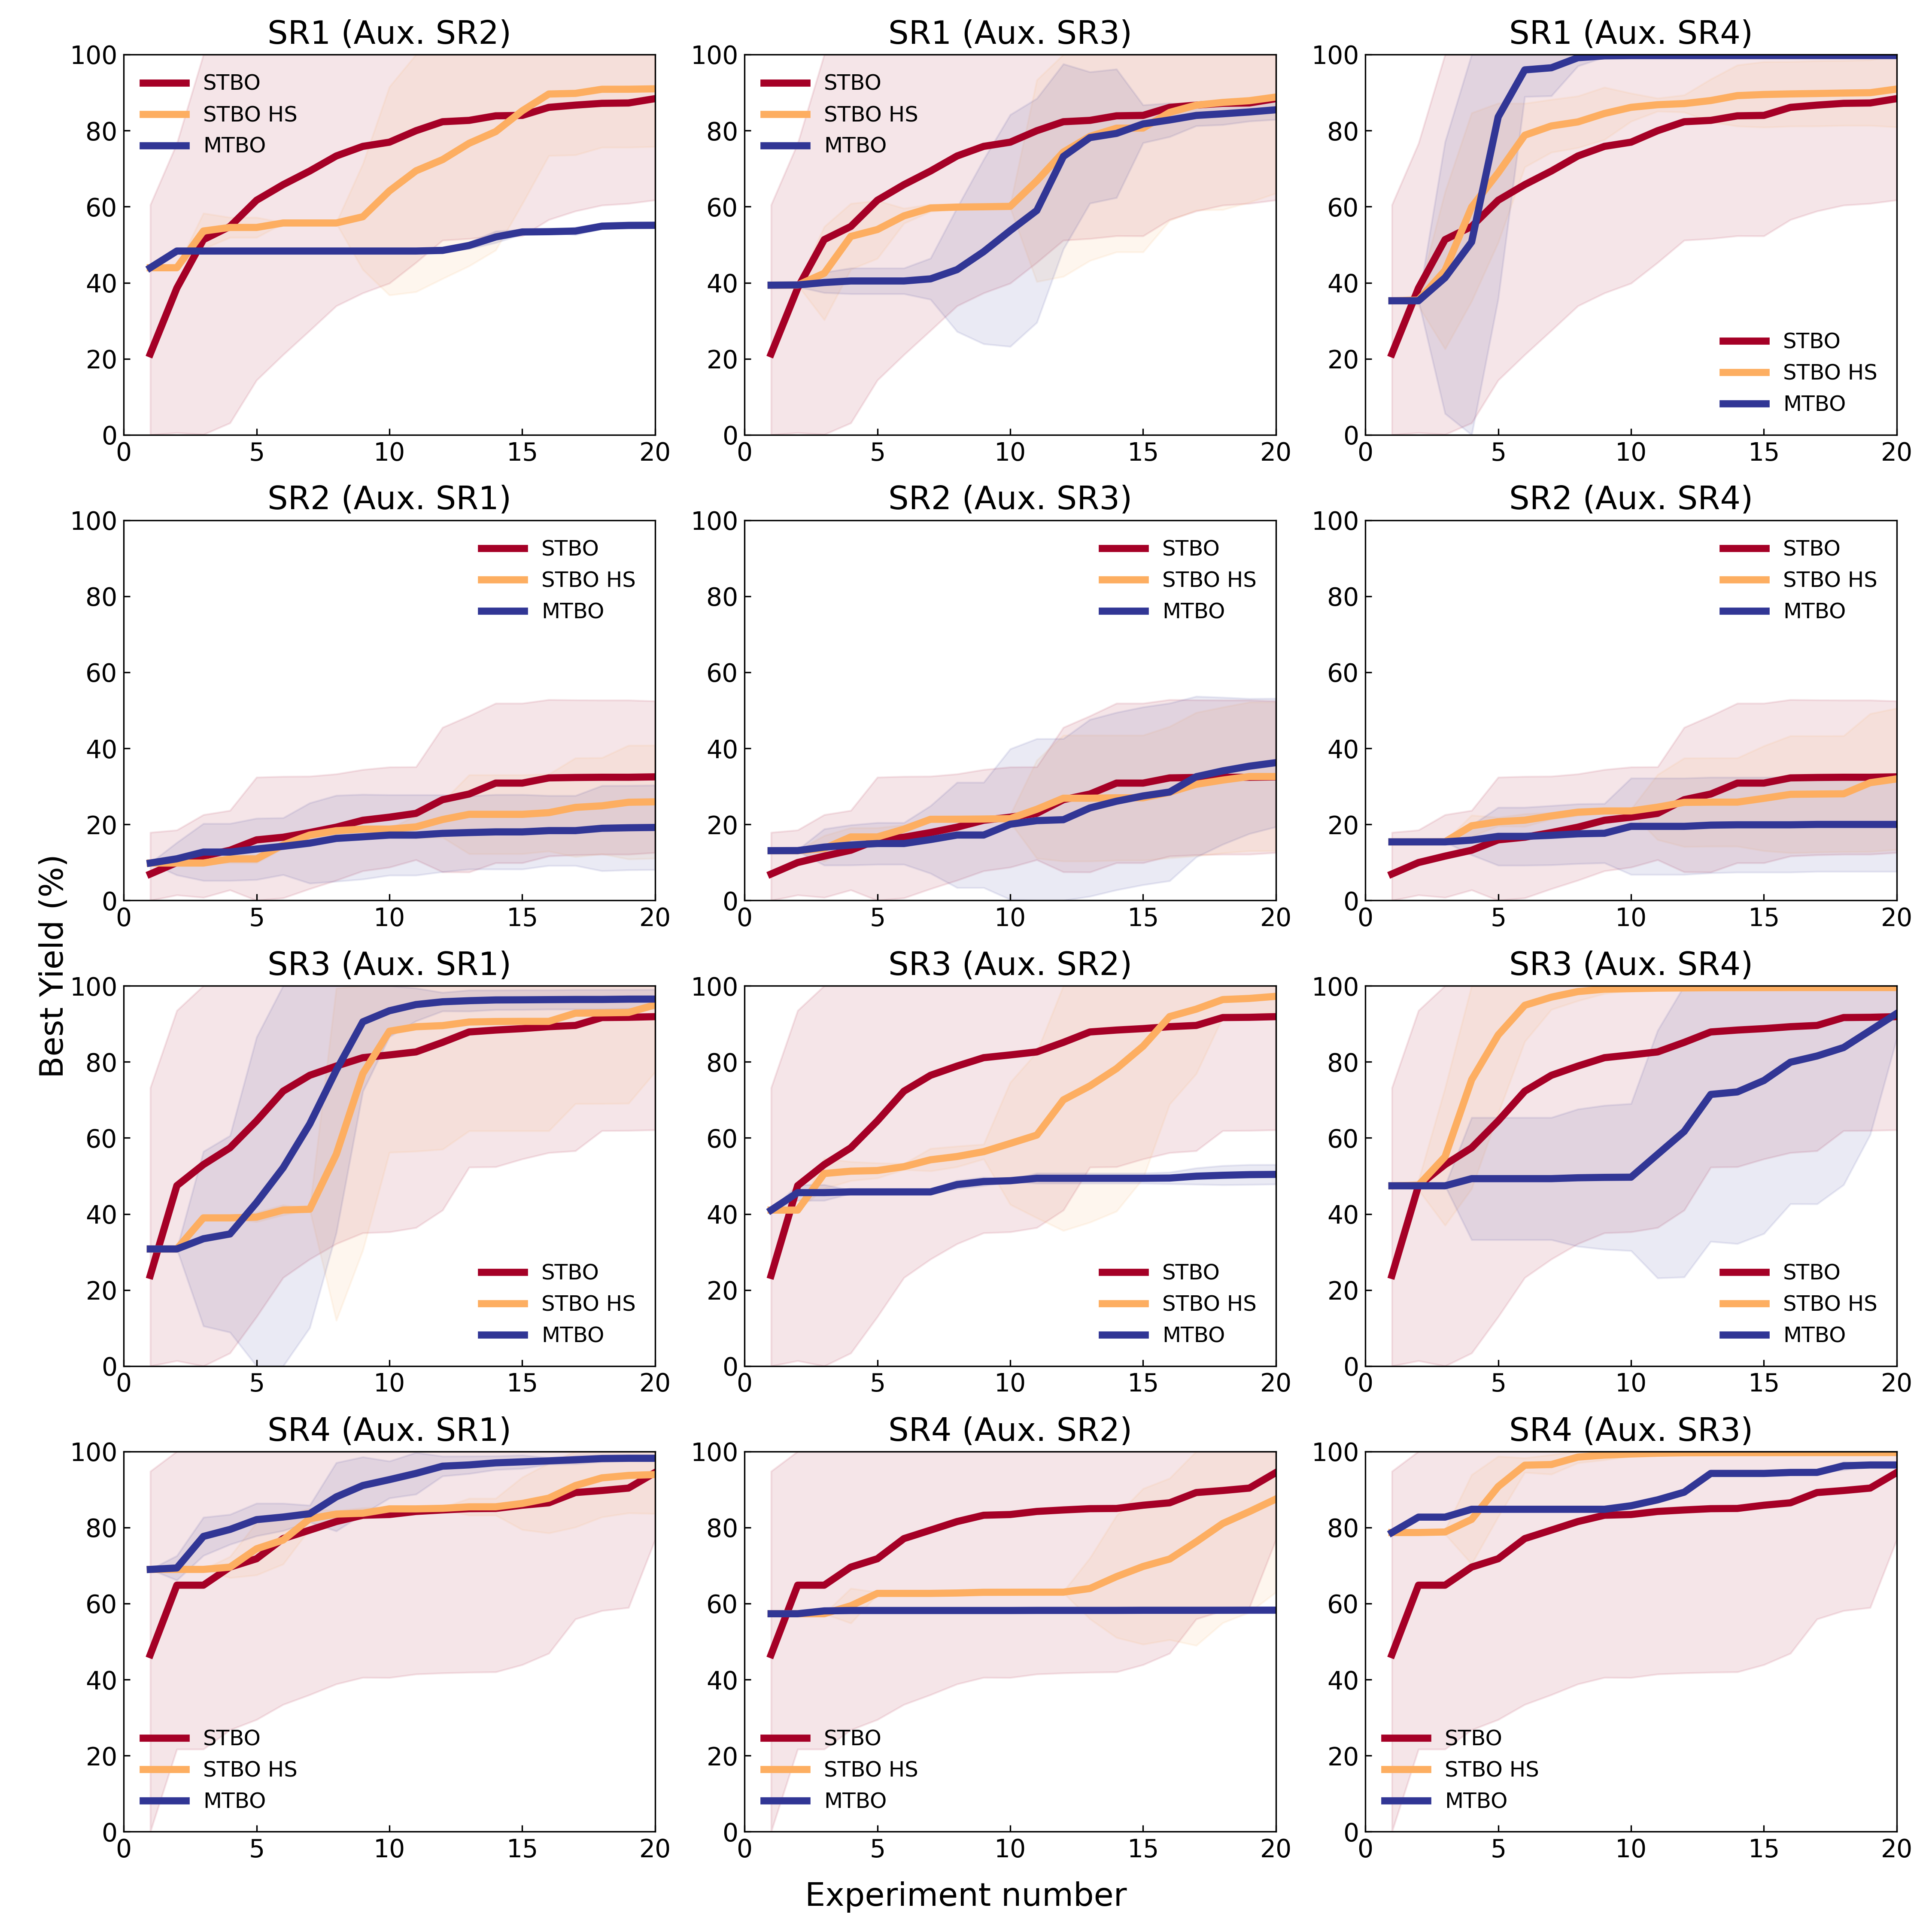
\includegraphics[width=1\textwidth]{gfx/Appendix/reizman_suzuki_reizman_suzuki_one_cotraining_optimization.png}
\label{fig:11}
\end{figure}

\begin{figure}
\caption{Comparison of the performance of single-task Bayesian optimization (STBO) and multi-task Bayesian optimization (MTBO) on Suzuki R1-R4 with Suzuki R1-R4 as auxiliary tasks. The text above the plot represents the data used as an auxiliary task.}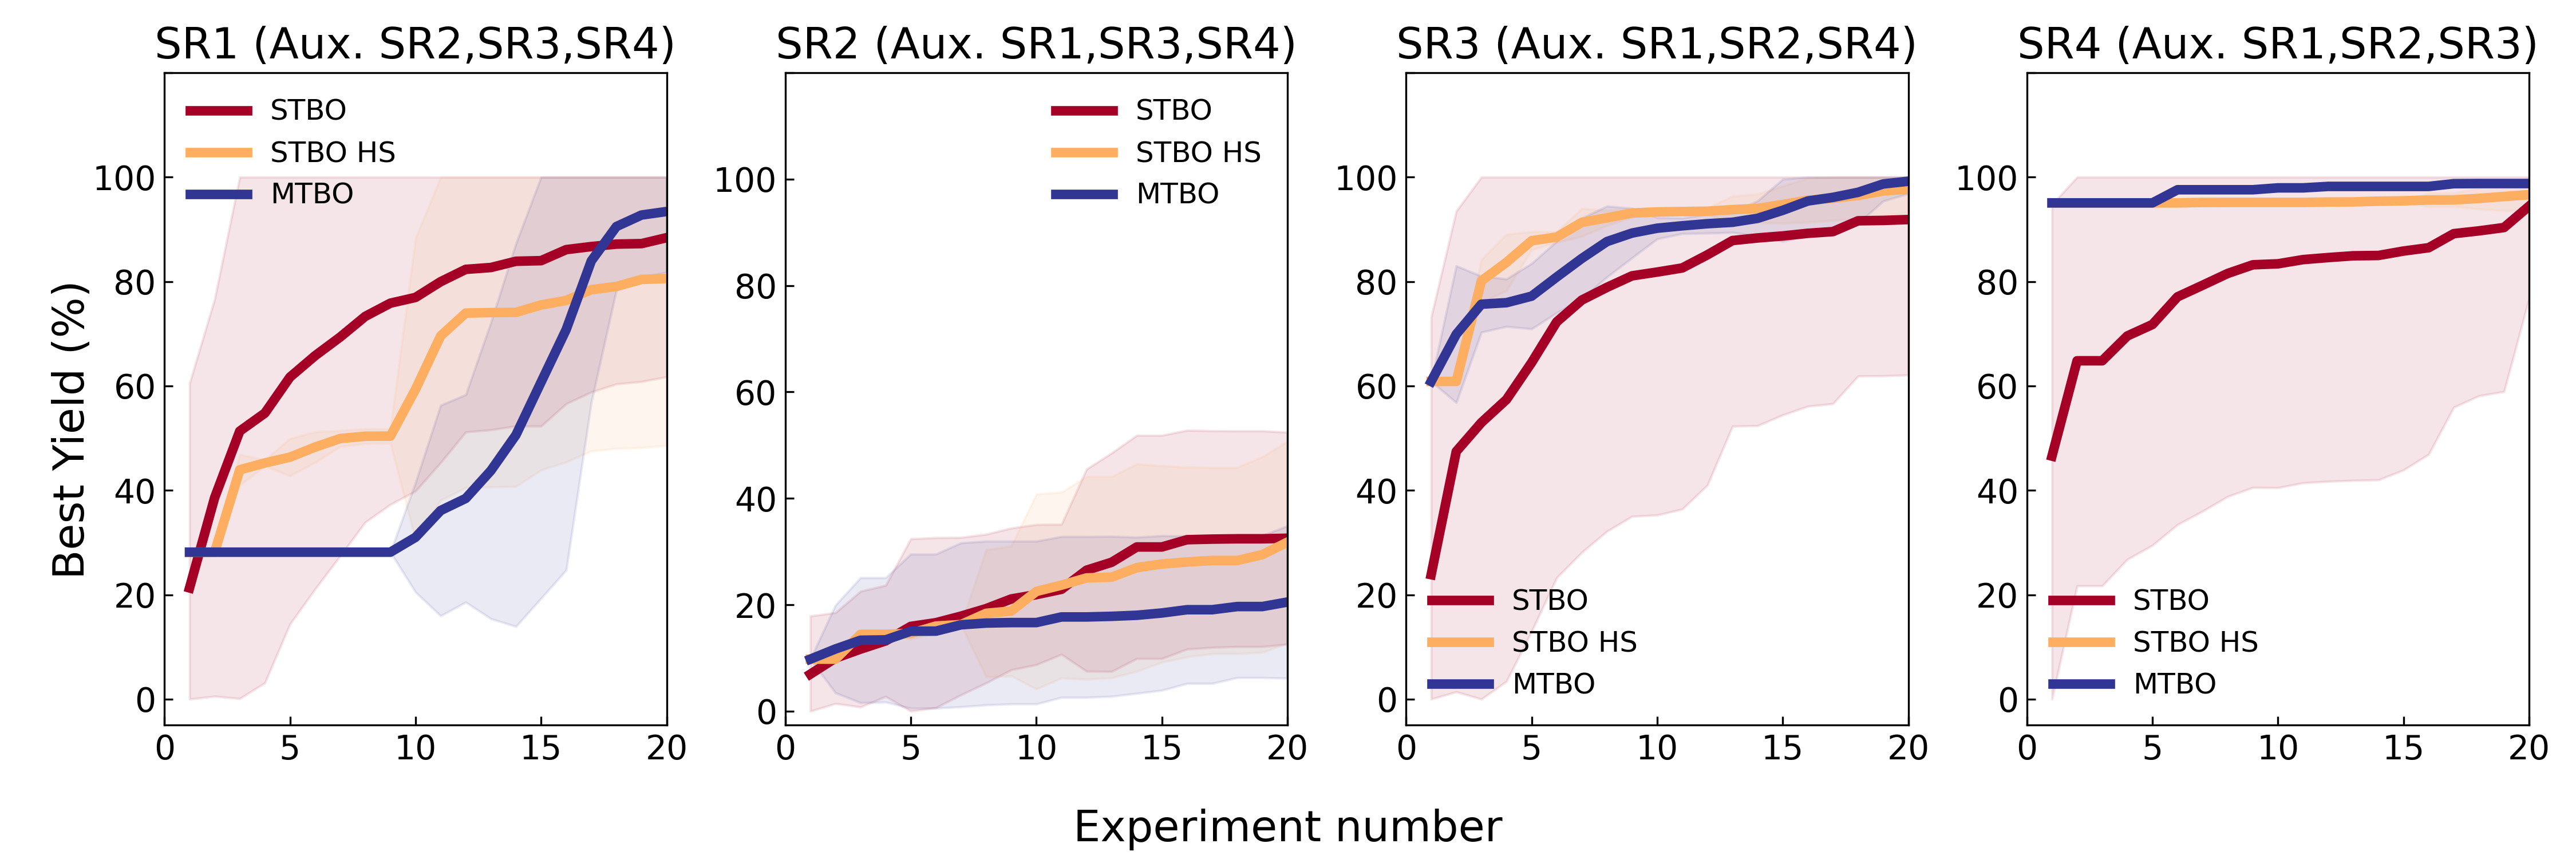
\includegraphics[width=1\textwidth]{gfx/Appendix/reizman_suzuki_baumgartner_suzuki_all_cotraining_optimization.png}
\label{fig:12}
\end{figure}

\subsection{C-N Benchmarks}

\begin{figure}
\caption{\textbf{Figure S14:} Comparison of the performance of single-task Bayesian optimization (STBO) and multi-task Bayesian optimization (MTBO) on C-N B1-B4 with C-N B1-B4 as auxiliary tasks. The text above the plot represents the data used as an auxiliary task.}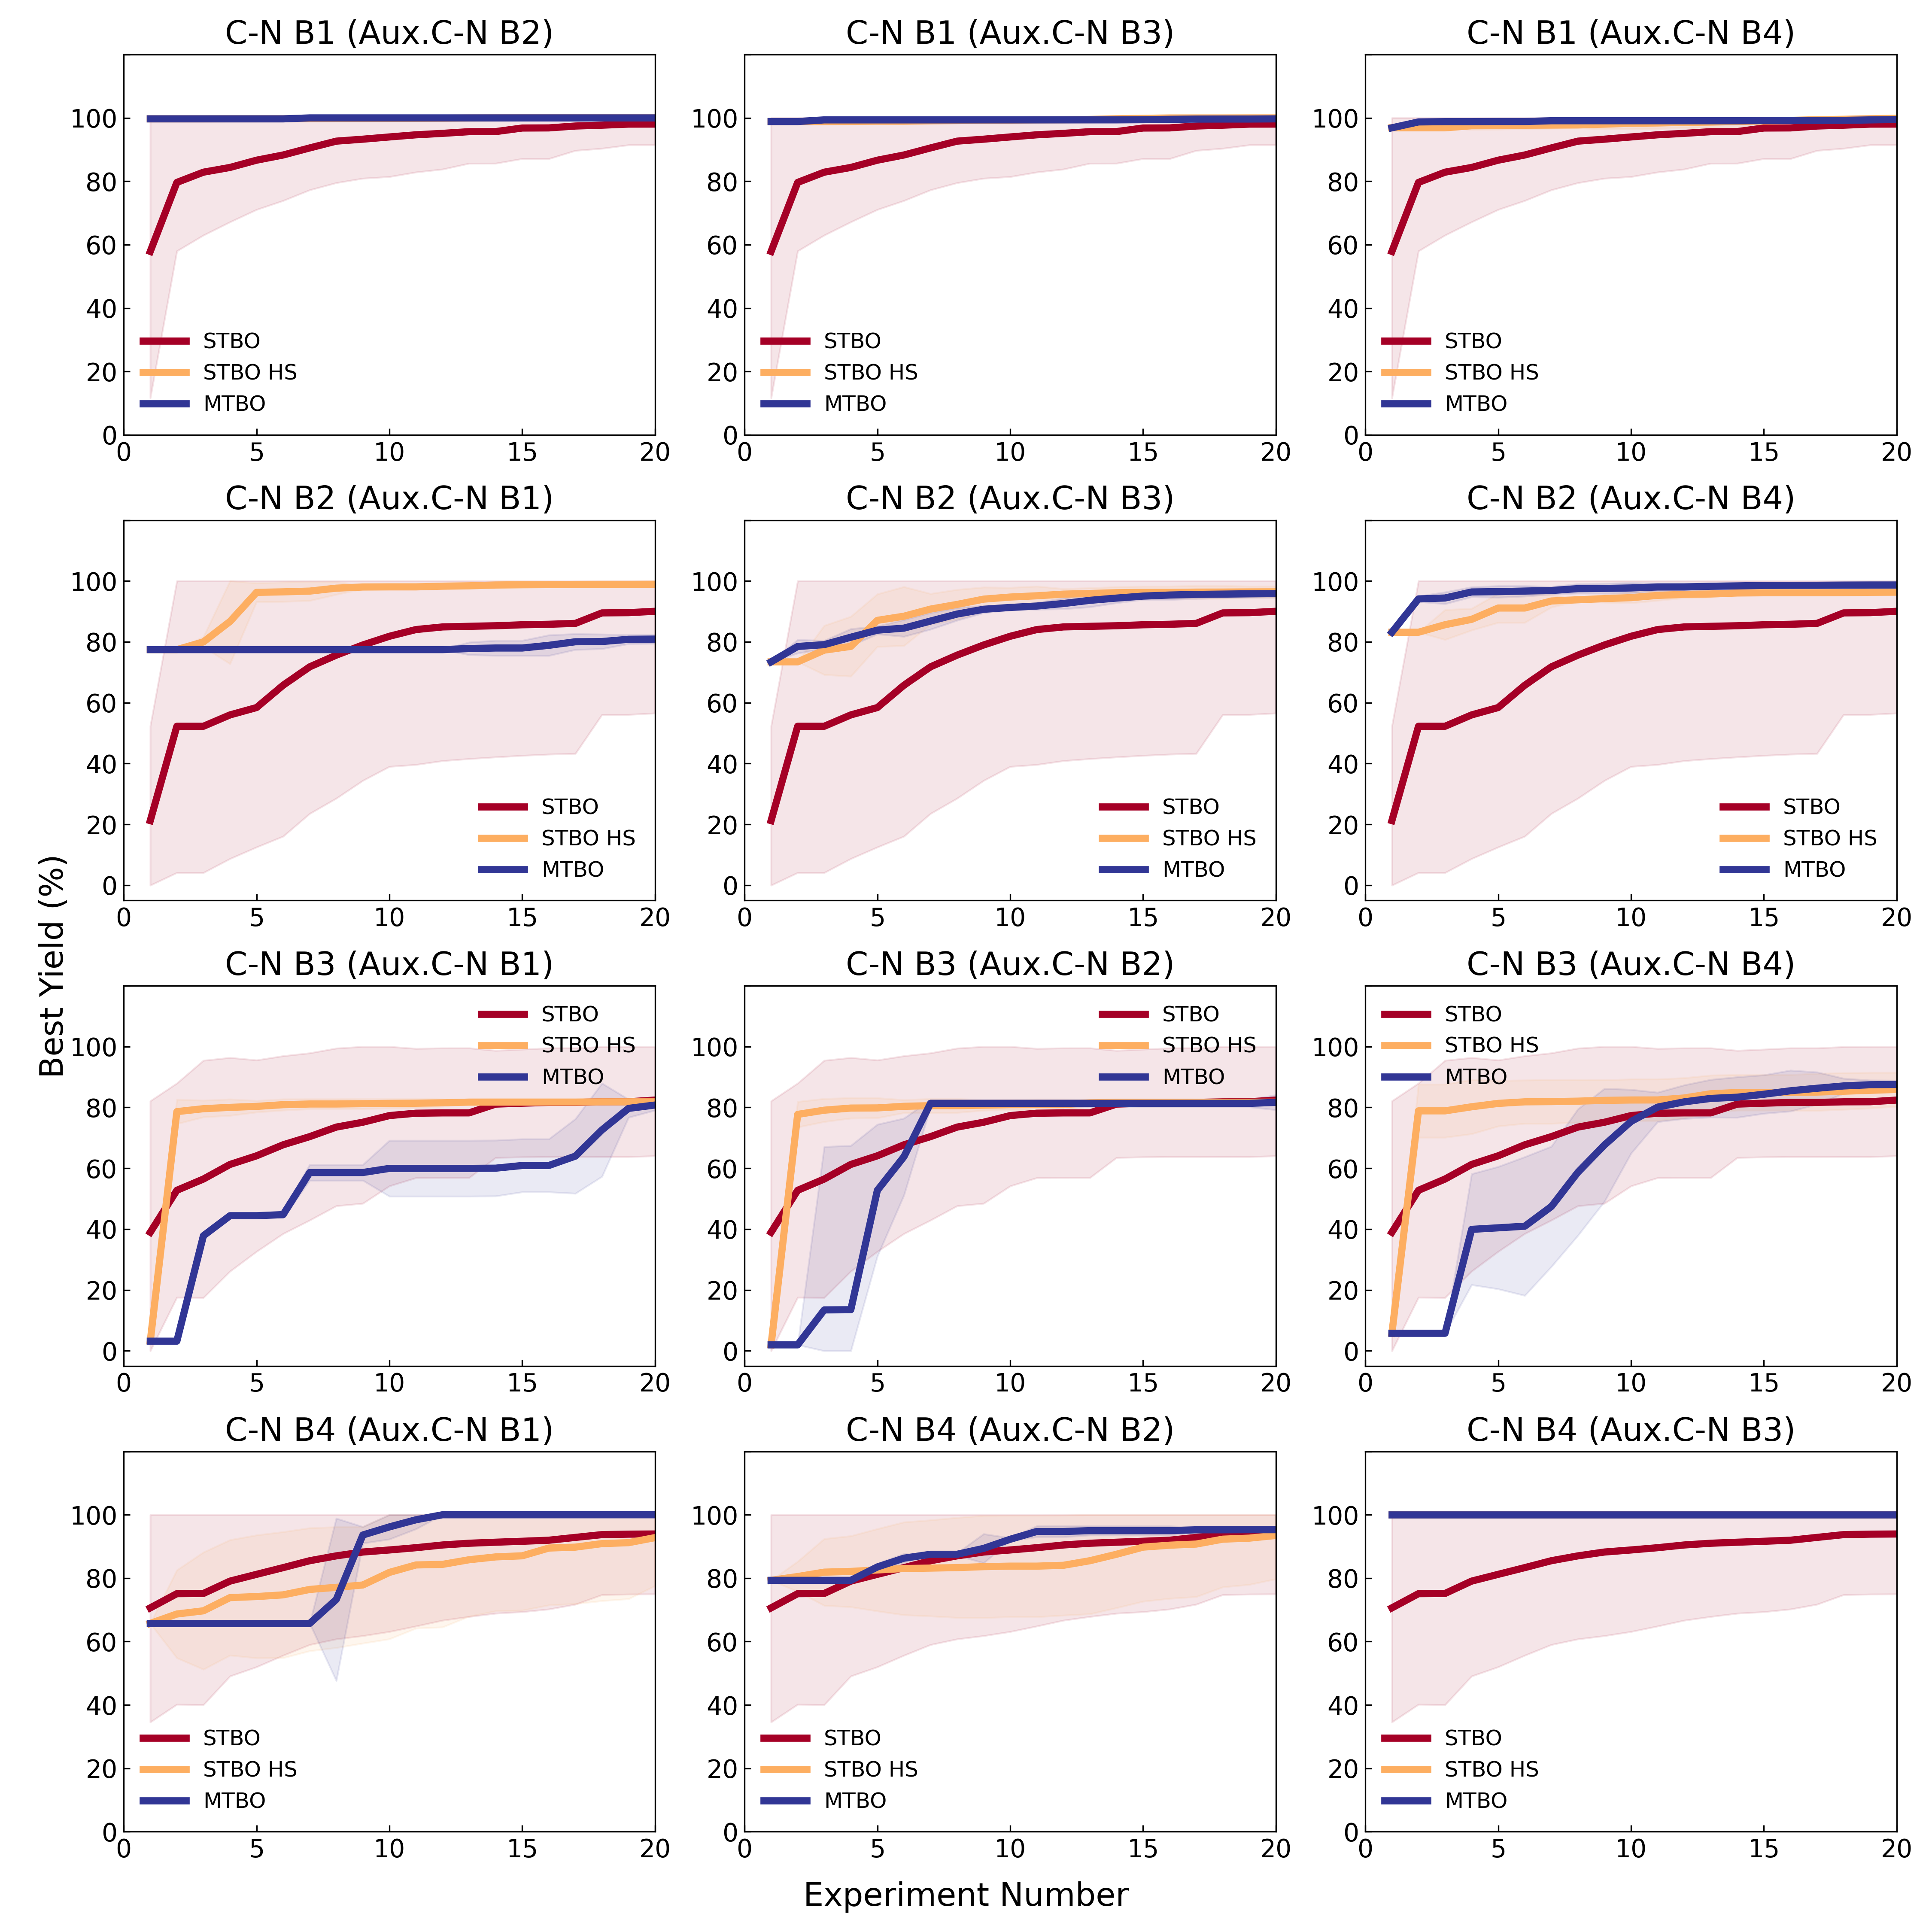
\includegraphics[width=1\textwidth]{gfx/Appendix/baumgartner_cn_baumgartner_cn_one_cotraining_optimization.png}
\label{fig:13}
\end{figure}

\begin{figure}
\caption{Comparison of the performance of single-task Bayesian optimization (STBO) and multi-task Bayesian optimization (MTBO) on C-N B1-B4 with all remaining C-N tasks for auxiliary training. The text above the plot represents the data used as an auxiliary task.}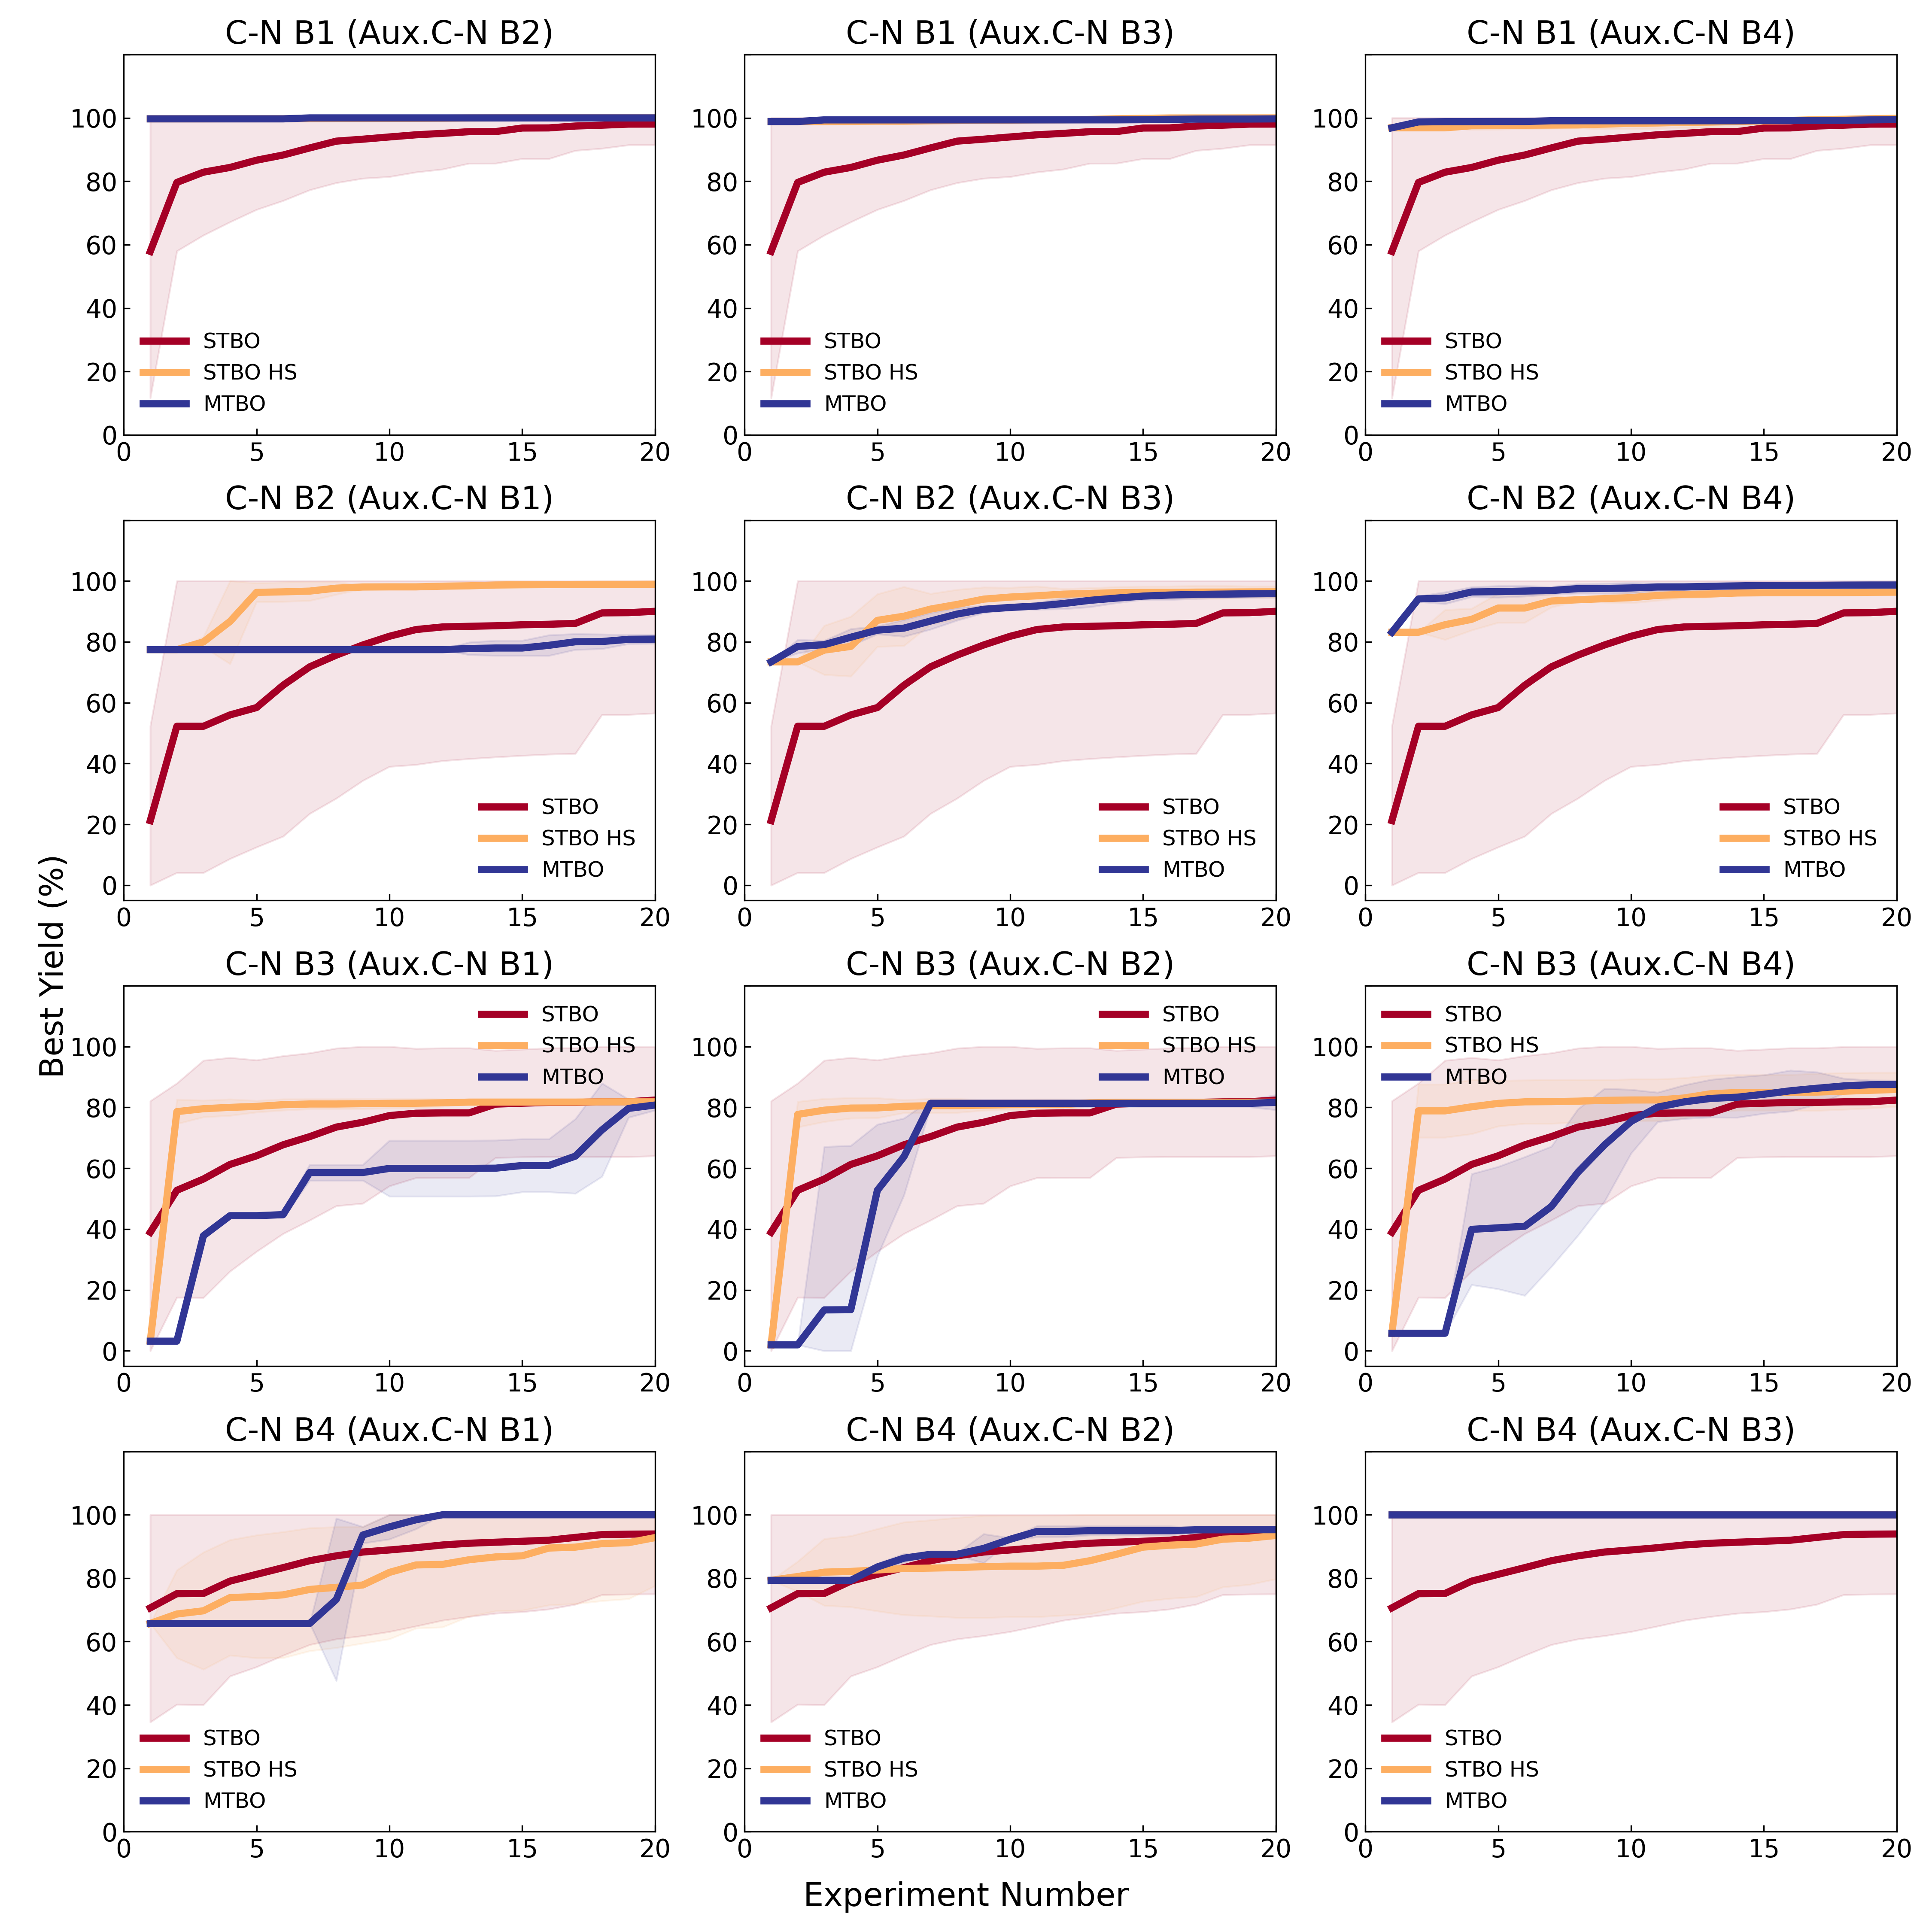
\includegraphics[width=1\textwidth]{gfx/Appendix/baumgartner_cn_baumgartner_cn_one_cotraining_optimization.png}
\label{fig:14}
\end{figure}


